% ============================================================================
%  VERIF-AI: A Deep Learning-Based Framework for Face-Based Deepfake Detection and Forensic Analysis
%  Project report (B.Tech, CSE - AI & DS, IIIT Senapati, Manipur).  Compile: latexmk -pdf Verif-AI_Project_Report.tex
%  Layout follows the department's reference report (A4, report class, grid tables with captions above, figure captions below,
%  numbered algorithms and listings, IEEE-style bibliography). Every figure, number and citation is traceable to the project repository.
% ============================================================================
\documentclass[11pt,a4paper]{report}

\usepackage[T1]{fontenc}
\usepackage{lmodern}
\usepackage{tgschola}% Century Schoolbook family, as in the reference report
\makeatletter
% small caps are not provided by Schola: imitate them the way the reference does (capital at full size, rest at 80 %)
\newcommand{\fsc}[2]{#1{\fontsize{\fpeval{0.8*\f@size}}{0}\selectfont #2}}
\makeatother

% ---- type sizes measured from the reference (internship) report: 11pt class scaled by 0.9265 (body 10.145 pt, leading 13.6 pt) ----
\makeatletter
\renewcommand\normalsize{\@setfontsize\normalsize{10.18}{12.0}%
  \abovedisplayskip 10\p@ \@plus2\p@ \@minus5\p@ \abovedisplayshortskip \z@ \@plus3\p@
  \belowdisplayshortskip 6\p@ \@plus3\p@ \@minus3\p@
  \belowdisplayskip \abovedisplayskip
  \let\@listi\@listI}
\renewcommand\small{\@setfontsize\small{9.30}{11}%
  \abovedisplayskip 8.5\p@ \@plus3\p@ \@minus4\p@ \abovedisplayshortskip \z@ \@plus2\p@
  \belowdisplayshortskip 4\p@ \@plus2\p@ \@minus2\p@ \def\@listi{\leftmargin\leftmargini \topsep 4\p@ \@plus2\p@ \@minus2\p@ \parsep 2\p@ \@plus\p@ \@minus\p@ \itemsep \parsep}%
  \belowdisplayskip \abovedisplayskip}
\renewcommand\footnotesize{\@setfontsize\footnotesize{8.37}{10}%
  \abovedisplayskip 6\p@ \@plus2\p@ \@minus4\p@ \abovedisplayshortskip \z@ \@plus\p@
  \belowdisplayshortskip 3\p@ \@plus\p@ \@minus2\p@ \def\@listi{\leftmargin\leftmargini \topsep 3\p@ \@plus\p@ \@minus\p@ \parsep 2\p@ \@plus\p@ \@minus\p@ \itemsep \parsep}%
  \belowdisplayskip \abovedisplayskip}
\renewcommand\scriptsize{\@setfontsize\scriptsize{7.44}{9.5}}
\renewcommand\tiny{\@setfontsize\tiny{5.58}{6}}
\renewcommand\large{\@setfontsize\large{11.16}{14}}
\renewcommand\Large{\@setfontsize\Large{13.39}{18}}
\renewcommand\LARGE{\@setfontsize\LARGE{16.07}{22}}
\renewcommand\huge{\@setfontsize\huge{19.27}{25}}
\renewcommand\Huge{\@setfontsize\Huge{23.13}{30}}
\makeatother
\usepackage[utf8]{inputenc}
\usepackage[a4paper,nohead,left=96pt,right=96pt,top=92pt,bottom=96pt,footskip=13pt]{geometry}
\usepackage{microtype}
\usepackage{setspace}
\usepackage{graphicx}
\usepackage{adjustbox}
\usepackage{needspace}
\usepackage{xcolor}
\usepackage{array,tabularx,multirow,booktabs,longtable}
\usepackage{float}
\usepackage{caption}
\usepackage{subcaption}
\usepackage{enumitem}
\usepackage{amsmath,amssymb}
\usepackage{url}
\usepackage{titlesec}
\usepackage{fancyhdr}
\usepackage{tocloft}
\usepackage{tikz}
\usetikzlibrary{arrows.meta,positioning,shapes.geometric,shapes.misc,fit,calc,backgrounds,decorations.pathreplacing,patterns}
\usepackage{pgfplots}
\pgfplotsset{compat=1.17}
\usepackage{algorithm}
\usepackage{algpseudocode}
\usepackage{listings}
\usepackage[numbers,sort&compress]{natbib}
\usepackage[hidelinks,pdftitle={VERIF-AI: A Deep Learning-Based Framework for Face-Based Deepfake Detection and Forensic Analysis},pdfauthor={Aniket Raj}]{hyperref}

% ---- look and feel (mirrors the reference report) ----
\setlength{\parindent}{17pt}
\setlength{\parskip}{0pt}
\renewcommand{\arraystretch}{1.15}
\captionsetup{font=small,labelfont=rm,labelsep=colon}
\captionsetup[table]{position=top}
\captionsetup[figure]{position=bottom}
\setlength{\cftfigindent}{0em}\setlength{\cfttabindent}{0em}
\setlist{itemsep=0.2ex,topsep=0.6ex,parsep=0pt}
\setcounter{tocdepth}{2}\setcounter{secnumdepth}{3}
\pagestyle{plain}
\sloppy
\emergencystretch=2em
\widowpenalty=10000 \clubpenalty=10000

\definecolor{codebg}{gray}{0.96}
\definecolor{accent}{HTML}{0F766E}
\definecolor{navy}{HTML}{0B2540}
\lstset{basicstyle=\ttfamily\fontsize{6.4}{7.3}\selectfont,backgroundcolor=\color{codebg},frame=single,rulecolor=\color{black!25},breaklines=true,
        breakatwhitespace=false,columns=fullflexible,keepspaces=true,numbers=left,numberstyle=\fontsize{5}{6}\selectfont\color{black!55},numbersep=5pt,
        xleftmargin=1.6em,framexleftmargin=1.6em,showstringspaces=false,captionpos=b,aboveskip=1.2ex,belowskip=0.8ex,
        keywordstyle=\bfseries,language=Python,morekeywords={self,True,False,None}}
\renewcommand{\lstlistingname}{Listing}
\renewcommand{\lstlistlistingname}{List of Listings}

% inline code that tolerates _ % # & in file names and identifiers
\newcommand{\code}[1]{\texttt{\detokenize{#1}}}
\newcommand{\pfake}{\ensuremath{P_{\mathrm{fake}}}}
\algrenewcommand\algorithmicrequire{\textbf{Input:}}
\algrenewcommand\algorithmicensure{\textbf{Output:}}
\floatname{algorithm}{Algorithm}


% ---- compact vertical rhythm (page-budget revision) ----
\makeatletter
\renewcommand\@makechapterhead[1]{\vspace*{8\p@}{\parindent \z@ \raggedright \normalfont
  \huge\bfseries \@chapapp\space \thechapter \par\nobreak \vskip 6\p@
  \interlinepenalty\@M \Huge \bfseries #1\par\nobreak \vskip 18\p@}}
\renewcommand\@makeschapterhead[1]{\vspace*{8\p@}{\parindent \z@ \raggedright \normalfont
  \interlinepenalty\@M \Huge \bfseries #1\par\nobreak \vskip 18\p@}}
\makeatother
\setlength{\floatsep}{8pt plus 2pt minus 2pt}
\setlength{\textfloatsep}{10pt plus 2pt minus 2pt}
\setlength{\intextsep}{8pt plus 2pt minus 2pt}
\setlength{\abovecaptionskip}{4pt}\setlength{\belowcaptionskip}{0pt}
\renewcommand{\topfraction}{0.9}\renewcommand{\bottomfraction}{0.9}\renewcommand{\textfraction}{0.08}\renewcommand{\floatpagefraction}{0.75}
\renewcommand{\cftchapafterpnum}{\vskip 2pt}
\setlength{\cftbeforechapskip}{4pt}\setlength{\cftbeforesecskip}{0pt}\setlength{\cftbeforesubsecskip}{0pt}\setlength{\cftbeforesubsubsecskip}{0pt}
\renewcommand{\cftsecfont}{\small}\renewcommand{\cftsecpagefont}{\small}
\renewcommand{\cftsubsecfont}{\small}\renewcommand{\cftsubsecpagefont}{\small}
\renewcommand{\cftsubsubsecfont}{\small}\renewcommand{\cftsubsubsecpagefont}{\small}
\renewcommand{\cftfigfont}{\footnotesize}\renewcommand{\cftfigpagefont}{\footnotesize}
\renewcommand{\cfttabfont}{\footnotesize}\renewcommand{\cfttabpagefont}{\footnotesize}
\setlength{\cftbeforefigskip}{0pt}\setlength{\cftbeforetabskip}{0pt}

\begin{document}
\raggedbottom

% ============================ FRONT MATTER (positions measured on the reference report; A4, 1 pt = 1 pt from the top-left corner) ============================
\newcommand{\pg}[2]{($(current page.north west)+(#1pt,-#2pt)$)}
\newcommand{\fmtext}[5]{% x, baseline y, anchor, width (0 = natural), content
  \node[anchor=#3,inner sep=0pt,outer sep=0pt,align=#5,text width=#4] at \pg{#1}{#2}}
\tikzset{fm/.style={inner sep=0pt,outer sep=0pt}}

% ============================ COVER ============================
\begin{titlepage}
\thispagestyle{empty}
\begin{tikzpicture}[remember picture,overlay,fm]
\node[anchor=north,text width=325pt,align=center,font=\fontsize{16.07}{16.1}\selectfont] at \pg{297.6}{151} {VERIF-AI: A Deep Learning-Based\\Framework for Face-Based Deepfake\\Detection and Forensic Analysis};
\node[anchor=base,font=\normalsize] at \pg{297.6}{301.5} {Submitted By};
\node[anchor=base,font=\Large] at \pg{297.6}{324.0} {\fsc{A}{NIKET} \fsc{R}{AJ}};
\node[anchor=base,font=\Large] at \pg{297.6}{341.9} {SEMESTER - VII};
\node[anchor=base,font=\Large] at \pg{297.6}{355.4} {230103030};
\node[anchor=base,font=\normalsize] at \pg{297.6}{375.8} {Under the Guidance of};
\node[anchor=base,font=\Large] at \pg{297.6}{396.8} {\fsc{D}{R}. \fsc{S}{UNITA} \fsc{W}{ARJRI}};
\node[anchor=north west] at \pg{226.3}{485} {
\includegraphics[width=141.7pt]{figures/iiit_manipur_logo.png}};
\node[anchor=base,font=\small] at \pg{297.6}{673.1} {\fsc{D}{EPARTMENT OF} \fsc{C}{OMPUTER} \fsc{S}{CIENCE AND} \fsc{E}{NGINEERING}};
\node[anchor=base,font=\small] at \pg{297.6}{685.2} {\fsc{I}{NDIAN} \fsc{I}{NSTITUTE OF} \fsc{I}{NFORMATION} \fsc{T}{ECHNOLOGY} \fsc{S}{ENAPATI}, \fsc{M}{ANIPUR}};
\node[anchor=base,font=\small] at \pg{297.6}{698.7} {\fsc{N}{OVEMBER}, 2026};
\end{tikzpicture}
\end{titlepage}

\pagenumbering{roman}
\setcounter{page}{1}

% ============================ DECLARATION ============================
\thispagestyle{plain}
\null
\begin{tikzpicture}[remember picture,overlay,fm]
\node[anchor=base,font=\fontsize{16.07}{20}\selectfont\bfseries] at \pg{297.6}{138} {Declaration};
\node[anchor=north west,text width=358pt,align=justify,font=\normalsize] at \pg{118}{157} {In this submission, I have expressed my idea in my own words, and I have adequately cited and referenced any ideas or words that were taken from another source. I also declare that I adhere to all principles of academic honesty and integrity and that I have not misrepresented or falsified any ideas, data, facts, or sources in this submission. If any violation of the above is made, I understand that the institute may take disciplinary action. Such a violation may also engender disciplinary action from the sources which were not properly cited or permission not taken when needed.};
\node[anchor=base,font=\normalsize] at \pg{396.6}{301.5} {ANIKET RAJ};
\node[anchor=base,font=\normalsize] at \pg{401.2}{314.9} {230103030};
\node[anchor=base west,font=\normalsize] at \pg{120.9}{357.1} {DATE:\ \raisebox{-1pt}{\rule{4.2cm}{0.4pt}}};
\end{tikzpicture}
\clearpage

% ============================ CERTIFICATE ============================
\thispagestyle{empty}
\null
\begin{tikzpicture}[remember picture,overlay,fm]
\node[anchor=north west] at \pg{117.9}{126.9} {
\includegraphics[width=51.2pt]{figures/iiit_manipur_logo.png}};
\node[anchor=base west,font=\normalsize] at \pg{178.2}{159.5} {Department of Computer Science and Engineering};
\node[anchor=base west,font=\normalsize] at \pg{178.2}{173.2} {Indian Institute of Information Technology Senapati, Manipur};
\draw[line width=0.4pt] \pg{117.4}{202.3} -- \pg{476.9}{202.3};
\node[anchor=base west,font=\normalsize] at \pg{118.1}{216.4} {Dr. Sunita Warjri};
\node[anchor=base east,font=\normalsize] at \pg{476.3}{216.4} {Email: sunitaw@iiitmanipur.ac.in};
\node[anchor=base west,font=\normalsize] at \pg{118.1}{230.1} {Assistant Professor};
\node[anchor=base east,font=\normalsize] at \pg{476.3}{230.1} {Contact No: +91 7085262822};
\node[anchor=base,font=\Huge\bfseries\itshape] at \pg{297.6}{276.2} {To Whom It May Concern};
\node[anchor=north,text width=358pt,align=center,font=\fontsize{11.16}{15.8}\selectfont] at \pg{297.6}{313.2} {\hyphenpenalty=10000\exhyphenpenalty=10000 \relax This is to certify that the project report entitled \textbf{``VERIF-AI: A Deep Learning-Based Framework for Face-Based Deepfake Detection and Forensic Analysis,''} submitted to the department of Computer Science and Engineering, Indian Institute of Information Technology Senapati, Manipur in partial fulfilment for the award of degree of Bachelor of Technology in Computer Science and Engineering (Specialisation: Artificial Intelligence and Data Science) is a record of bonafide work carried out by \textbf{Aniket Raj} bearing roll number \textbf{230103030}.};
\node[anchor=base,font=\fontsize{11.16}{15.8}\selectfont] at \pg{391}{507.8} {Signature of Supervisor};
\node[anchor=base,font=\fontsize{11.16}{15.8}\selectfont\bfseries] at \pg{387}{529.8} {(Dr. Sunita Warjri)};
\foreach \i in {1,2,3,4}{
  \pgfmathsetmacro{\yy}{568.5+(\i-1)*24}
  \node[anchor=base west,font=\normalsize,text width=290pt,align=left] at \pg{118.3}{\yy} {Signature of the Examiner \i\ \dotfill\null};
}
\end{tikzpicture}
\clearpage

% ============================ ABSTRACT ============================
\chapter*{\centering Abstract}
Synthetic face imagery produced by generative adversarial networks, face-swapping tools and diffusion models can now be hard to
distinguish from genuine photographs, which creates a demand for forensic tools that give not only a verdict but also inspectable evidence.
This report presents \textbf{Verif-AI}, an end-to-end framework for face-based deepfake detection and forensic analysis that works on both
images and videos. Faces are located with MTCNN and passed to a two-stream convolutional classifier: an EfficientNet-B0 stream that
reads the RGB face, and a second EfficientNet-B0 stream that reads a noise residual produced by a fixed three-kernel Spatial Rich Model
(SRM) filter bank. The two feature vectors are fused by a small classification head into a single raw sigmoid score. Gradient-weighted
Class Activation Mapping (Grad-CAM) shows which facial regions influenced the RGB stream's score, a video pipeline adds face tracking,
frame-level timelines, suspicious time ranges and stored evidence frames, and a PDF forensic report records the result together with the
model checkpoint hash and the limitations. The system is implemented as a FastAPI backend and a React/TypeScript dashboard in which
uploads are deleted immediately after analysis and stored results can be deleted by the user.

The evaluation is reported as it was obtained, including its negative findings. The selected production model (v2, trained on a sample of
the DeepFakeFace dataset) reaches an accuracy of 0.875 and a ROC-AUC of 0.941 on held-out identities seen-generator data, but only 0.746 and 0.849 on an
unseen text-to-image generator, and it falsely flags genuine video from the Celeb-DF dataset at chance level. Diagnostic experiments
traced this failure to an image-quality shortcut in the training data, and adding Celeb-DF video frames and quality augmentation (Model 4)
raised the video-level accuracy on held-out Celeb-DF identities to 0.980, which is within-dataset evidence only. A further experiment
with modern-generator faces (E3) detected held-out fakes of those generators almost perfectly, but without a generator-disjoint test it
cannot be read as evidence of general detection, and it did not meet the pre-registered promotion rule. Scores are raw sigmoid outputs,
not calibrated probabilities. The latest model, E4, is the default of the local examiner demonstration; it did not pass the promotion rule, so the public deployment still serves v2. The report does not claim a general detector of AI-generated images or videos, and the public deployment on
free hosting tiers runs in a restricted mode that is not production-ready.

\medskip\noindent\textbf{Keywords:} deepfake detection, two-stream network, EfficientNet, SRM noise residuals, Grad-CAM, digital forensics, FastAPI, React.

\clearpage

% ============================ ACKNOWLEDGEMENT ============================
\chapter*{\centering Acknowledgement}
I would like to express my deep gratitude to my supervisor, Dr.\ Sunita Warjri, Assistant Professor, Department of Computer Science and Engineering, IIIT Manipur, for her guidance and support throughout this project.
Her feedback shaped both the system design and the way the results are evaluated and reported, and her encouragement made it possible to
take on the more demanding parts of the work, in particular the careful treatment of evaluation leakage and of what the system can and
cannot claim.

The two-stream design that Verif-AI builds on started from an earlier Forensic-Net prototype by Lakshya Singh, whose notebook, checkpoint
and plots are preserved in the project repository; the web application, the training and evaluation tooling and the analysis in this
report were developed on top of that starting point. I am grateful to the authors and maintainers of the open datasets and software used
here (DeepFakeFace, Celeb-DF v2, FFHQ, SFHQ, PyTorch, FastAPI and React), to Kaggle for the free GPU time on which the models were
trained, and to the Indian Institute of Information Technology Senapati, Manipur, for providing the environment in which this work was carried out.

\vspace{1.5cm}
\begin{flushright}
Aniket Raj\\
Roll No: 230103030\\
IIIT Manipur
\end{flushright}

\clearpage

% ============================ CONTENTS ============================
\renewcommand{\contentsname}{Contents}
\tableofcontents
\clearpage
\phantomsection\addcontentsline{toc}{chapter}{List of Figures}
\listoffigures
\phantomsection\addcontentsline{toc}{chapter}{List of Tables}
\listoftables
\clearpage

\pagenumbering{arabic}
\setcounter{page}{1}

\chapter{Introduction}
\label{ch:intro}

\section{Introduction}
Photographs and video of a person's face have long served as informal evidence of identity and events. Generative models have weakened
that assumption: generative adversarial networks (GANs) \citep{goodfellow2014gan,karras2019stylegan}, face-swapping and re-enactment
tools \citep{rossler2019ff} and, more recently, diffusion models \citep{ho2020ddpm,rombach2022ldm} can produce or alter faces whose
artefacts are invisible to the naked eye. Research on \emph{media forensics} \citep{verdoliva2020media,tolosana2020deepfakes} responds
with automatic detectors, but a detector that only prints ``fake'' or ``real'' is of limited use to a reviewer: the verdict has to be accompanied
by evidence that can be inspected, by the conditions under which it is reliable, and by an honest statement of what it cannot decide.

\emph{Verif-AI} is a software system built around that idea. It accepts an image or a video, finds the faces in it, scores every face with a
two-stream convolutional network, shows which facial regions influenced the score, summarises a video over time and generates a PDF
forensic report. This report describes the design, the implementation, and --- with equal weight --- the evaluation of the system,
including the experiments that showed where it fails.

\subsection{Problem Statement: Verifying Faces in an Age of Synthetic Media}
The practical problem has three parts.

\begin{enumerate}
\item \textbf{Detection.} Given a face crop, estimate whether it shows a photographed face or a generated or manipulated one. Detectors
trained on one family of manipulations often transfer poorly to another \citep{wang2020cnn,ojha2023universal,corvi2023diffusion}, so the
measured accuracy depends heavily on how the test data relate to the training data.
\item \textbf{Evidence.} A score alone does not let a reviewer judge a result. The system must localise what drove the decision, report the
detection confidence of the face finder, show where in a video suspicious frames occur and keep a record (file hash, model checkpoint,
settings) that makes the analysis reproducible.
\item \textbf{Honesty and privacy.} Neural scores are not probabilities of authenticity \citep{guo2017calibration}, detectors are exposed to
\emph{shortcuts} in their training data \citep{geirhos2020shortcut}, and uploaded media can be sensitive. The system must therefore say
``inconclusive'' when it cannot decide, avoid presenting scores as certainties, and delete uploads after use.
\end{enumerate}

\begin{figure}[ht]
\centering
\begin{adjustbox}{max width=\linewidth,center}
\begin{tikzpicture}[font=\small,node distance=0.45cm and 0.6cm,
  box/.style={draw,rounded corners=2pt,minimum height=0.9cm,align=center,fill=white},
  io/.style={draw,rounded corners=2pt,minimum height=0.9cm,align=center,fill=navy!8},
  arr/.style={-{Stealth[length=2mm]},thick}]
\node[io] (in) {Image or\\video};
\node[box,right=of in] (det) {Face\\detection\\(MTCNN)};
\node[box,right=of det] (model) {Two-stream\\classifier};
\node[io,right=of model] (out) {Verdict, score,\\Grad-CAM, report};
\draw[arr] (in)--(det); \draw[arr] (det)--(model); \draw[arr] (model)--(out);
\node[box,below=0.6cm of model,fill=accent!12] (ev) {Evidence: heat-maps, timeline, face tracks, PDF report};
\draw[arr,dashed] (model)--(ev);
\end{tikzpicture}
\end{adjustbox}
\caption[Conceptual overview of Verif-AI]{Conceptual overview of Verif-AI. A face is located, scored by a two-stream network and returned together with inspectable
evidence. Scores are raw model outputs (not probabilities); INCONCLUSIVE is an explicit outcome.}
\label{fig:overview}
\end{figure}

\subsection{Motivation and Project Objectives}
The project started from an earlier prototype that combined an RGB and an SRM noise stream and reported very high accuracy on a single
dataset. When the prototype's checkpoint was evaluated on independent, identity-disjoint data it performed at chance level, which made the
central motivation of this work concrete: \emph{a detector is only as trustworthy as its evaluation}. The objectives were therefore both
engineering and scientific:

\begin{itemize}
\item \textbf{Objective 1:} to re-implement the two-stream detector as a clean, tested software package that loads the original
checkpoints and a newly trained one, with identical preprocessing for training and inference.
\item \textbf{Objective 2:} to train and evaluate the model with identity-disjoint splits, duplicate removal, validation-only model
selection and a clear separation of internal and cross-generator evaluation.
\item \textbf{Objective 3:} to provide explainable output --- Grad-CAM heat-maps, face-level scores, video timelines, face tracks and a PDF report --- through an
API and a web dashboard, with privacy-preserving handling of uploads.
\item \textbf{Objective 4:} to investigate honestly where the model fails (for example on genuine video) and to document the cause and the
limits of every claim.
\item \textbf{Objective 5:} to deploy a public demonstration (static frontend, hosted API) and to state its restrictions truthfully.
\end{itemize}

\subsection{Scope and Target Applications}
Verif-AI analyses \emph{faces}. It is intended for educational demonstration, exploratory review of suspicious face media by a human and
research on detector generalisation. It is \textbf{not} a general detector of AI-generated images or videos, does not analyse non-face content,
does not establish authorship or provenance, and a ``real'' result is not proof of authenticity. Scores are uncalibrated; these boundaries decide how
every number in Chapter~\ref{ch:results} may be read.

\subsection{Contributions}
\begin{enumerate}
\item A tested two-stream detection package with a documented preprocessing pipeline that reproduces training-time cropping, JPEG
round-trip and normalisation at inference time (Chapters~\ref{ch:design} and~\ref{ch:impl}).
\item An image and video analysis service with Grad-CAM evidence, face tracking, frame timelines, PDF reports and deletion
(Chapter~\ref{ch:impl}), and a dashboard with original, heat-map and overlay views.
\item An evaluation record that includes an identified failure (chance-level behaviour on genuine video), a diagnosis of its cause as an
image-quality shortcut, a pre-registered acceptance gate and modern-generator experiments (Chapter~\ref{ch:results}).
\item A reproducible training and data-review workflow (Kaggle GPU notebooks that export only checkpoints and metrics) and a dataset
licence review that did not accept licence badges as proof (Chapter~\ref{ch:results} and Appendix~\ref{app:datasets}).
\end{enumerate}

\subsection{Organisation of the Report}
Chapter~\ref{ch:lit} surveys the field, the research gap and the contributions of this work; Chapter~\ref{ch:req} the requirements and technology stack;
Chapter~\ref{ch:design} the architecture, model and pipelines; Chapter~\ref{ch:impl} their implementation, testing and deployment;
Chapter~\ref{ch:results} the experiments, their interpretation and limitations; Chapter~\ref{ch:concl} the conclusion and future work.
Appendices~\ref{app:code}--\ref{app:datasets} give key source code, the API and configuration, and the dataset review.

\chapter{Literature Survey}
\label{ch:lit}

\section{Literature Survey}
This chapter summarises the research that Verif-AI builds on and the open problems that shaped its evaluation. It is not a complete survey;
broader reviews are given by Verdoliva \citep{verdoliva2020media} and Tolosana et al.\ \citep{tolosana2020deepfakes}.

\subsection{Evolution of Deepfake Generation and Detection}
\textbf{Generation.} Generative adversarial networks \citep{goodfellow2014gan} made photorealistic face synthesis practical;
StyleGAN and its successors generate high-resolution faces from a latent code \citep{karras2019stylegan,karras2020stylegan2}. Face-swapping
and re-enactment methods transfer one person's face or expression onto another's video, and the FaceForensics++ benchmark collects four
such manipulation families \citep{rossler2019ff}. Diffusion models \citep{ho2020ddpm}, in particular latent diffusion
\citep{rombach2022ldm}, now produce images from text prompts and can inpaint or edit regions of real photographs, so a single dataset
may contain fully synthetic, edited and swapped faces.

\textbf{Detection.} Early detectors used compact convolutional networks on face crops, such as MesoNet \citep{afchar2018mesonet}, or
general-purpose backbones such as Xception \citep{chollet2017xception} that performed best in the FaceForensics++ study
\citep{rossler2019ff}. Two-stream networks combine an RGB stream with a stream that sees low-level traces: Zhou et al.\
\citep{zhou2017twostream} paired a face-classification stream with a steganalysis-features stream for tampered faces, and constrained
convolutional layers \citep{bayar2016constrained} learn high-pass filters for manipulation detection. Dang et al.\ \citep{dang2020detection}
add attention maps that localise manipulated regions. Large benchmark efforts such as Celeb-DF \citep{li2020celebdf} and the DFDC
collection \citep{dolhansky2020dfdc} made video-level evaluation possible.

\subsection{Theoretical Framework of Modern Forensics}
\textbf{RGB versus noise residuals.} A generator leaves statistical traces in the high-frequency content of an image that are largely
independent of the depicted face. Rich-model steganalysis \citep{fridrich2012srm} extracts such traces by applying fixed high-pass
\emph{residual} filters and analysing the co-occurrence of the residuals. Verif-AI uses a fixed bank of three $3\times3$ high-pass
kernels (Chapter~\ref{ch:design}) that suppress image content and leave a noise residual for a second convolutional stream. The filters
are not trained, which keeps the stream's input independent of the training data.

\textbf{EfficientNet.} EfficientNet \citep{tan2019efficientnet} scales depth, width and resolution of a convolutional network with a
compound coefficient. The smallest member, EfficientNet-B0, has about 5.3 million parameters and reports 77.1\% ImageNet top-1
accuracy, which makes two parallel copies affordable on a CPU.

\textbf{Grad-CAM.} Gradient-weighted Class Activation Mapping \citep{selvaraju2017gradcam} weights the activation maps of a chosen
convolutional layer by the average gradient of the class score with respect to them and shows the result as a coarse heat-map. The map
indicates regions that increased the score; it is an explanation of the \emph{model}, not evidence that those pixels were altered
\citep{selvaraju2017gradcam}. Figure~\ref{fig:srm-concept} contrasts the information seen by the two streams.

\begin{figure}[ht]
\centering
\begin{adjustbox}{max width=\linewidth,center}
\begin{tikzpicture}[font=\small,x=1cm,y=1cm]
\foreach \i/\t/\c in {0/{RGB face (what a person sees)}/navy!10, 1/{High-pass residual (what the SRM stream sees)}/accent!10}{
  \node[draw,minimum width=3.7cm,minimum height=3.0cm,fill=\c] at (4.4*\i,0) {};
  \node[align=center,font=\footnotesize,text width=3.6cm] at (4.4*\i,-2.1) {\t};
}
\foreach \a in {0,...,7}{\foreach \b in {0,...,5}{
  \pgfmathtruncatemacro{\w}{20+mod(\a*7+\b*13,5)*10}
  \fill[navy!\w] ({-1.8+\a*0.46},{1.35-\b*0.5}) rectangle ++(0.42,0.46);
}}
\foreach \a in {0,...,31}{\foreach \b in {0,...,23}{
  \pgfmathtruncatemacro{\v}{(mod(\a*17+\b*29+\a*\b,7)>5) ? 40 : 6}
  \fill[accent!\v] ({2.6+\a*0.115},{1.4-\b*0.12}) rectangle ++(0.1,0.1);
}}
\draw[-{Stealth},thick] (1.9,0)--(2.5,0);
\end{tikzpicture}
\end{adjustbox}
\caption[Illustration (schematic, not a real face) of the idea behind the two streams: the RGB stream]{Illustration (schematic, not a real face) of the idea behind the two streams: the RGB stream sees image content, whereas the fixed
SRM-style filters remove content and leave a high-frequency noise residual in which generator traces may remain.}
\label{fig:srm-concept}
\end{figure}

\subsection{Analysis of Benchmark Architectures}
Table~\ref{tab:backbones} compares backbones commonly used for face-manipulation detection. The figures are the sizes and ImageNet
results reported by the original papers; they describe the architectures, not their forensic accuracy, which depends on training data.

\begin{table}[ht]
\centering
\caption{Backbones used in the deepfake-detection literature (published figures).}
\label{tab:backbones}
\small
\begin{adjustbox}{max width=\linewidth,center}
\begin{tabular}{|l|c|c|p{5.2cm}|}
\hline
\textbf{Architecture} & \textbf{Params (M)} & \textbf{ImageNet top-1} & \textbf{Relevance} \\ \hline
MesoNet (Meso-4) \citep{afchar2018mesonet} & 0.028 & -- & Very small network designed for face-video forgery \\ \hline
Xception \citep{chollet2017xception} & 22.9 & 79.0\% & Strongest baseline in FaceForensics++ \citep{rossler2019ff} \\ \hline
ResNet-50 \citep{he2016resnet} & 25.6 & -- & Common general-purpose baseline \\ \hline
\textbf{EfficientNet-B0} \citep{tan2019efficientnet} & \textbf{5.3} & \textbf{77.1\%} & Used for both streams of Verif-AI \\ \hline
\end{tabular}
\end{adjustbox}
\end{table}

\subsection{Comparison of Forensic Datasets}
Table~\ref{tab:datasets} lists the datasets that matter for this project. Their \emph{construction} matters as much as their size: how real and
fake samples are paired, whether identities repeat across splits, and how fakes were compressed or processed all create shortcuts that a
detector can learn instead of the manipulation itself (Section~\ref{sec:shortcuts}).

\begin{table}[ht]
\centering
\caption[Datasets referenced in this work (figures as stated by the dataset papers or by the dataset]{Datasets referenced in this work (figures as stated by the dataset papers or by the dataset documentation in the repository).}
\label{tab:datasets}
\small
\begin{adjustbox}{max width=\linewidth,center}
\begin{tabular}{|p{2.6cm}|p{3.0cm}|p{2.9cm}|p{3.4cm}|}
\hline
\textbf{Dataset} & \textbf{Content} & \textbf{Fakes} & \textbf{Use in Verif-AI} \\ \hline
FaceForensics++ \citep{rossler2019ff} & 1{,}000 original videos & 4 manipulation methods & Cited; not used (access agreement) \\ \hline
DFDC \citep{dolhansky2020dfdc} & over 100{,}000 clips & Several methods & Cited; not used \\ \hline
Celeb-DF v2 \citep{li2020celebdf} & 590 real and 5{,}639 fake videos & Face swap (one method) & Video-level training and test (research use only) \\ \hline
DeepFakeFace \citep{song2023dff} & 30{,}000 real (IMDB-WIKI) photographs \citep{rothe2018imdbwiki} & 3$\times$30{,}000: inpainting, face swap, text-to-image & Primary training data (sampled subset) \\ \hline
FFHQ \citep{karras2019stylegan} & 70{,}000 real faces & -- & Real faces in experiment E3 \\ \hline
SFHQ \citep{sfhq2022} & Synthetic faces & StyleGAN-generated & Fake faces in experiment E3 \\ \hline
\end{tabular}
\end{adjustbox}
\end{table}

\subsection{Generalisation, Shortcuts and Calibration}
\label{sec:shortcuts}
\textbf{Generalisation.} A classifier trained on images from one generator can be nearly perfect on that generator and weak on others.
Wang et al.\ \citep{wang2020cnn} found that a classifier trained on one GAN with suitable augmentation generalised surprisingly well to
other CNN-based generators, while stressing the limits of that result; Ojha et al.\ \citep{ojha2023universal} and Corvi et al.\ \citep{corvi2023diffusion} study the transfer between GAN and diffusion generators, where detectors trained on one family often degrade on
the other. A reliable evaluation therefore needs a held-out \emph{generator}, not only held-out images.

\textbf{Shortcut learning.} Geirhos et al.\ \citep{geirhos2020shortcut} describe how networks solve benchmarks with unintended cues.
In deepfake data the cue may be image sharpness, resolution, file format, compression history or the source of the real class.
Chapter~\ref{ch:results} documents a concrete case in this project.

\textbf{Calibration and explanation.} The sigmoid output of a modern network is usually over-confident
\citep{guo2017calibration}; Verif-AI therefore labels it a \emph{model score} and never a probability. Grad-CAM maps are explanations of
the model's decision, and as noted above they do not prove manipulation.

\subsection{Synthesis and Research Gap}
Prior work supplies the ingredients --- an efficient backbone, a noise-residual stream, class-activation explanations and benchmark
datasets --- but a practical forensic tool also needs a consistent preprocessing pipeline, video aggregation, privacy-preserving
handling of uploads and an evaluation that distinguishes internal from cross-generator behaviour. The gap addressed in this report is
therefore less a new architecture than a \emph{complete and honestly evaluated system}: the two-stream design is kept, while the data
splits, leakage checks, failure diagnosis and the limits of each claim are treated as first-class results.


\section{Research Gap, Project Contributions, and Novelty}
\label{sec:novelty}
This section states what existing work has achieved, which gaps matter for this project, which components are borrowed, and what Verif-AI itself contributes. \textbf{Verif-AI does not propose a new deep-learning architecture}, and it does not claim to have invented EfficientNet, SRM filtering, MTCNN or Grad-CAM; its contributions are in engineering, system integration and experimental method.

\subsection{What existing research has achieved}
Benchmarks and generators: FaceForensics++ \citep{rossler2019ff}, Celeb-DF \citep{li2020celebdf}, the DFDC dataset \citep{dolhansky2020dfdc} and DeepFakeFace \citep{song2023dff} supply labelled data. Detectors: compact and Xception-style CNNs \citep{afchar2018mesonet,rossler2019ff}; two-stream networks that combine an RGB branch with a low-level residual branch \citep{zhou2017twostream}; detectors that exploit high-frequency/SRM-filtered features to generalise across forgeries \citep{luo2021highfreq}; blending-boundary cues for unseen manipulations \citep{li2020facexray}; recurrent video models over frame features \citep{guera2018rnn,masi2020twobranch}; and detectors studied across generators \citep{wang2020cnn,ojha2023universal,corvi2023diffusion}. Explanation: Grad-CAM \citep{selvaraju2017gradcam}. Evaluation caveats: shortcut learning \citep{geirhos2020shortcut} and over-confident scores \citep{guo2017calibration}. Surveys: \citep{verdoliva2020media,tolosana2020deepfakes}.

\subsection{Gaps that matter for this project}
\begin{enumerate}[label=G\arabic*.]
\item The cited papers present \emph{methods and benchmark results}; they are not described as ready-to-use tools that return per-face evidence, video timelines and a record of which model and file produced a result.
\item Reported accuracy depends on the split. Identity-disjoint, duplicate-free and generator-disjoint testing, and the check that an apparent skill is not a quality shortcut, must be done again for any new system.
\item Video support is usually a temporal classifier validated inside one dataset; a deployed tool also needs face tracking, aggregation and honest handling of frames for which no evidence was stored.
\item A prototype inherited by this project (Forensic-Net, Section~\ref{sec:prototype}) reported very high accuracy that could not be reproduced on independent data, so the model itself needed to be re-trained and re-evaluated.
\end{enumerate}

\subsection{Established components used (not new)}
EfficientNet-B0 \citep{tan2019efficientnet} as both backbones; the three SRM-style high-pass kernels after Fridrich and Kodovsk\'y \citep{fridrich2012srm}; the two-stream idea of an image branch plus a low-level residual branch \citep{zhou2017twostream}; MTCNN \citep{zhang2016mtcnn}; Grad-CAM \citep{selvaraju2017gradcam}; ImageNet initialisation, AdamW \citep{loshchilov2019adamw} and PyTorch \citep{paszke2019pytorch}; and the public datasets of Chapter~\ref{ch:results}.

\subsection{The prototype and what Verif-AI adds}
\label{sec:prototype}
The RGB + three-kernel SRM two-stream design, with its feature concatenation and sigmoid head, comes from the earlier Forensic-Net prototype written by Lakshya Singh (notebook, checkpoint and plots preserved in the repository). That prototype analysed only the first frame of a file and had no application, no leakage-controlled evaluation and no tests. Everything listed below was developed for Verif-AI.

\begin{table}[ht]
\centering
\caption[Existing work and how Verif-AI relates to it (only capabilities stated in the cited papers or]{Existing work and how Verif-AI relates to it (only capabilities stated in the cited papers or in this repository).}
\label{tab:novelty}
\small
\begin{tabular}{|p{3.3cm}|p{3.9cm}|p{5.6cm}|}
\hline
\textbf{Existing work} & \textbf{What it contributes} & \textbf{Verif-AI: implemented / extended / different} \\ \hline
Zhou et al.\ \citep{zhou2017twostream} & two-stream face-tampering detector (image + low-level branch) & uses the two-stream idea with fixed SRM residuals; adds identity-disjoint training/evaluation and a per-quality-bin gate \\ \hline
Fridrich \& Kodovsk\'y \citep{fridrich2012srm} & rich residual models for steganalysis & three fixed kernels as the noise stream; examines when that stream carries a quality shortcut (Section~\ref{sec:diag}) \\ \hline
Luo et al.\ \citep{luo2021highfreq}; Li et al.\ \citep{li2020facexray} & generalisation through high-frequency features / blending boundaries & not re-implemented; the project measures generalisation with an unseen-generator split instead \\ \hline
G\"uera \& Delp \citep{guera2018rnn}; Masi et al.\ \citep{masi2020twobranch} & recurrent networks over frame features for video & different approach: per-face scores, IoU face tracks, per-track median, suspicious segments and stored evidence frames (unvalidated aggregation rule) \\ \hline
Selvaraju et al.\ \citep{selvaraju2017gradcam} & Grad-CAM & applied to the RGB stream, shown with Original/Heatmap/Overlay views, stored for evidence frames, stated as not proof \\ \hline
Wang et al., Ojha et al., Corvi et al.\ \citep{wang2020cnn,ojha2023universal,corvi2023diffusion} & detectors studied across generators & motivates the internal vs.\ cross-generator reporting; no claim of universal detection \\ \hline
Celeb-DF, DeepFakeFace, FFHQ/SFHQ \citep{li2020celebdf,song2023dff,karras2019stylegan,sfhq2022} & datasets & used under their licences; leakage control, near-duplicate removal and a licence review before use \\ \hline
\end{tabular}
\end{table}

\subsection{Contributions, by type}
\begin{description}
\item[Research novelty.] None claimed at the level of a new architecture or algorithm. The research-level results are empirical findings: (i) the production model was at chance on held-out Celeb-DF video; (ii) image sharpness is a measurable shortcut in DeepFakeFace and the noise stream carries it; (iii) a per-quality-bin acceptance gate (validated with synthetic controls) fails all four candidate models although two pass the usual ROC-AUC screen.
\item[Engineering novelty.] Training-matched preprocessing (JPEG round-trip), strict checkpoint loading with hash recording, an INCONCLUSIVE band and decisiveness value, atomic job storage, privacy-preserving deletion, memory-aware lite mode, and a model registry (default / alternative / rollback) with per-result model identification.
\item[System-level integration.] One React + FastAPI application that turns the two-stream model into an inspectable workflow: face detection, image and video analysis, face tracking, Grad-CAM, timelines, evidence frames, downloadable PDF forensic report, history and deletion, deployed as a static frontend plus a hosted API.
\item[Experimental contribution.] A reproducible Kaggle training and evaluation workflow with pre-registered protocols; four models compared under identical code (Table~\ref{tab:fourvideo}); experiments E1--E4 including a frozen promotion rule; E4 as the latest model, with its limits reported (Section~\ref{sec:e4}).
\end{description}

\subsection{What remains limited}
No new detector architecture, no validation of the video aggregation rule on labelled videos, no calibration, no claim about AI-generated video, E4 not approved by the promotion rule, and the live deployment serves v2 (Chapter~\ref{ch:results}, Section~\ref{sec:limits}).



\chapter{Requirement Engineering}
\label{ch:req}

\section{Requirement Engineering and Design}
The transition from a research prototype to a usable forensic tool requires explicit requirements. They were derived from three sources:
the weaknesses found when the earlier prototype was evaluated, the needs of a reviewer who must trust and audit a result, and the
constraints of free hardware and open datasets. This chapter states them and the resulting technology choices.

\subsection{Project Feasibility Analysis}
\textbf{Technical feasibility.} Two EfficientNet-B0 networks (about 12 million parameters together) run on a CPU: a single image is
analysed in roughly 0.5--2.5 seconds on the development laptop, and a video of a few seconds in several seconds (measured values from the
analysis records). Training needs a GPU, which was obtained from the free Kaggle Tesla T4 allowance; one training run takes between about
one and several hours depending on the amount of data.

\textbf{Operational feasibility.} The system is delivered as a Docker image or as two parts (static React build and a Python API), uses no
external AI service or API key, and needs no account for the end user.

\textbf{Economic feasibility.} All software is open source, and training and hosting used free tiers. The free hosting tier limits what the
public demonstration can do (Section~\ref{sec:deploy-impl}); a plan with more memory would be required for the full feature set.

\textbf{Legal and ethical feasibility.} Face data are personal data. The system deletes uploads right after analysis, avoids a public list
of other users' analyses, and was developed with datasets whose terms were reviewed (Appendix~\ref{app:datasets}). Datasets with research-only
terms are used for non-commercial study only.

\textbf{Main risks.} (i) Over-optimistic evaluation because of leakage or shortcuts; (ii) a detector that fails on genuine video or on new
generators; (iii) over-interpretation of scores or heat-maps by users. They are addressed by the evaluation design of
Chapter~\ref{ch:results} and by the wording of the user interface.

\subsection{Requirements Analysis}
\textbf{Stakeholders.} (1) A \emph{reviewer} who uploads media and needs a verdict with inspectable evidence; (2) a \emph{student or researcher}
who wants a reproducible detector for experiments; (3) an \emph{operator} who deploys and maintains the service.

\begin{table}[ht]
\centering
\caption{Functional requirements (FR) of Verif-AI.}
\label{tab:fr}
\small
\begin{adjustbox}{max width=\linewidth,center}
\begin{tabular}{|p{1.0cm}|p{8.6cm}|p{2.3cm}|}
\hline
\textbf{ID} & \textbf{Requirement} & \textbf{Status} \\ \hline
FR-1 & Accept an image or a video through one upload control; detect the media type automatically; reject unsupported or oversized files with a clear message. & Implemented \\ \hline
FR-2 & Detect faces with a published detector and analyse every sufficiently large and confident face (up to 10 per image). & Implemented \\ \hline
FR-3 & Score each face with the two-stream model and return a raw fake score in $[0,1]$ together with a REAL / FAKE / INCONCLUSIVE label. & Implemented \\ \hline
FR-4 & Report ``no usable face'' as INCONCLUSIVE rather than as real or fake. & Implemented \\ \hline
FR-5 & Provide Grad-CAM heat-maps for faces and for evidence frames; show original, heat-map and overlay views. & Implemented (when the host allows) \\ \hline
FR-6 & For video: sample frames, track faces, aggregate per track, list suspicious time ranges and store the highest-scoring frames as evidence. & Implemented \\ \hline
FR-7 & Show the frame-level score timeline and let the user select a frame and see its stored image and heat-map. & Implemented \\ \hline
FR-8 & Generate a PDF forensic report with the verdict, scores, file hash, model checkpoint hash, evidence and limitations. & Implemented \\ \hline
FR-9 & Run video analysis as a background job with progress reporting. & Implemented \\ \hline
FR-10 & Let the user view earlier analyses and delete a result at any time; delete uploads immediately after analysis; expire results automatically. & Implemented \\ \hline
FR-11 & Expose model information (name, architecture, checkpoint hash, thresholds, limits) through the API and the interface. & Implemented \\ \hline
FR-12 & Provide documented REST endpoints with typed error responses and a health check. & Implemented \\ \hline
FR-13 & Detect modern text-to-image and diffusion-edited faces and AI-generated video reliably. & \textbf{Not achieved} (see Chapter~\ref{ch:results}) \\ \hline
\end{tabular}
\end{adjustbox}
\end{table}

\begin{table}[ht]
\centering
\caption{Non-functional requirements (NFR) and how each was addressed or measured.}
\label{tab:nfr}
\small
\begin{adjustbox}{max width=\linewidth,center}
\begin{tabular}{|p{2.4cm}|p{5.0cm}|p{4.6cm}|}
\hline
\textbf{Category} & \textbf{Requirement} & \textbf{Measure / mechanism} \\ \hline
Performance & An image is analysed within a few seconds on a CPU; video does not block the browser. & Measured 0.5--2.5\,s per image on the development laptop; video runs as a polled background job. \\ \hline
Resource use & Run on a modest machine. & Measured on the laptop: about 490\,MB after the model loads, about 780\,MB peak for one image with Grad-CAM, over 820\,MB while analysing a video. \\ \hline
Privacy & Do not retain uploads or expose other users' analyses. & Uploads deleted right after analysis; results expire (72\,h default); the global history list can be disabled; results are reachable only by a 128-bit random identifier. \\ \hline
Security & Resist malformed and malicious uploads. & Extension allow-list, size and pixel limits, decoding check, server-chosen file names, CORS restricted to configured origins. \\ \hline
Honesty & Never present a score as a probability or a heat-map as proof. & Fixed wording in the interface and report; INCONCLUSIVE band; limitation text on every result. \\ \hline
Reproducibility & The result must be traceable to a model and an input. & File SHA-256 and checkpoint SHA-256 stored in every result and report. \\ \hline
Portability & Run on Windows, Linux and in a container. & Docker image; CPU and CUDA paths; environment-variable configuration. \\ \hline
Maintainability & Changes must be verifiable. & Automated tests: 152 backend tests passed (7 environment-gated skips), 63 frontend unit tests and 9 browser end-to-end tests at the time of writing. \\ \hline
Usability & Work on desktop, tablet and phone. & Responsive layout verified at 1440, 1024, 768, 390 and 320\,px widths. \\ \hline
\end{tabular}
\end{adjustbox}
\end{table}

\subsection{Proposed System Architecture}
The system is organised in three tiers (Figure~\ref{fig:dfd}): a browser dashboard, an HTTP API, and the analysis core. The
data-flow diagram follows a single request from upload to result. Detailed designs of the model and the pipelines are in
Chapter~\ref{ch:design}.

\begin{figure}[ht]
\centering
\begin{adjustbox}{max width=\linewidth,center}
\begin{tikzpicture}[font=\footnotesize,
  ext/.style={draw,rectangle,minimum width=1.9cm,minimum height=0.8cm,align=center,fill=black!6},
  proc/.style={draw,rounded corners=3pt,minimum width=2.3cm,minimum height=0.9cm,align=center,fill=navy!7},
  store/.style={draw,minimum width=2.3cm,minimum height=0.7cm,align=center,fill=accent!10,
     path picture={\draw[black!60] ([xshift=0.25cm]path picture bounding box.north west)--([xshift=0.25cm]path picture bounding box.south west);}},
  arr/.style={-{Stealth[length=1.8mm]},thick}]
\node[ext] (user) at (0,0) {User\\(browser)};
\node[proc] (api) at (4.0,0) {1. Validate and\\receive upload};
\node[proc] (face) at (8.3,0) {2. Detect faces\\(MTCNN)};
\node[proc] (net) at (8.3,-2.3) {3. Score faces\\(two-stream net)};
\node[proc] (agg) at (4.0,-2.3) {4. Aggregate\\(image / video)};
\node[proc] (ev) at (4.0,-4.6) {5. Evidence:\\Grad-CAM, frames};
\node[store] (res) at (8.3,-4.6) {D1 Results and\\evidence images};
\node[proc] (pdf) at (0,-4.6) {6. PDF report};
\draw[arr] (user)--node[above,font=\scriptsize]{media file}(api);
\draw[arr] (api)--node[above,font=\scriptsize]{decoded media}(face);
\draw[arr] (face)--node[right,font=\scriptsize]{face crops}(net);
\draw[arr] (net)--node[above,font=\scriptsize]{fake scores}(agg);
\draw[arr] (agg)--node[right,font=\scriptsize]{selected faces/frames}(ev);
\draw[arr] (ev)--node[above,font=\scriptsize]{artifacts}(res);
\draw[arr] (agg.west)--++(-1.0,0)|-(user.south east);
\node[font=\scriptsize,align=center,fill=white,inner sep=1pt] at (1.2,-2.3) {verdict,\\scores};
\draw[arr] (res.south)--++(0,-0.6)-|(pdf.south);
\node[font=\scriptsize,fill=white,inner sep=1pt] at (4.0,-5.2) {read};
\draw[arr] (pdf)--(user);
\node[font=\scriptsize,fill=white,inner sep=1pt,xshift=0.35cm] at (0,-2.3) {PDF};
\draw[arr,dashed] (api.south west)--++(-0.3,-0.3)node[left,font=\scriptsize,align=center]{upload\\deleted};
\end{tikzpicture}
\end{adjustbox}
\caption[Data-flow diagram of Verif-AI. Processes 1--6 run in the API process; D1 is the results store (evidence images and JSON), which is deleted on request or after the retention period]{Data-flow diagram of Verif-AI. Processes 1--6 run in the API process; D1 is the results store (evidence images and JSON), which is
deleted on request or after the retention period. The original upload is deleted as soon as processing 4 finishes.}
\label{fig:dfd}
\end{figure}

\begin{figure}[ht]
\centering
\begin{adjustbox}{max width=\linewidth,center}
\begin{tikzpicture}[font=\footnotesize,
  uc/.style={draw,ellipse,minimum width=3.6cm,minimum height=0.75cm,align=center,fill=navy!6},
  act/.style={draw,rectangle,minimum width=1.6cm,minimum height=0.8cm,align=center,fill=black!6}]
\draw[rounded corners=4pt,dashed] (2.6,-5.6) rectangle (10.4,1.0);
\node[font=\scriptsize\bfseries] at (6.5,0.75) {Verif-AI system};
\node[act] (rev) at (0.5,-2.0) {Reviewer};
\node[act] (op) at (12.2,-2.0) {Operator};
\node[uc] (u1) at (6.5,0.1) {Upload image or video};
\node[uc] (u2) at (6.5,-0.9) {View verdict and scores};
\node[uc] (u3) at (6.5,-1.9) {Inspect heat-map and overlay};
\node[uc] (u4) at (6.5,-2.9) {Browse video timeline and frames};
\node[uc] (u5) at (6.5,-3.9) {Download PDF report};
\node[uc] (u6) at (6.5,-4.9) {Delete analysis};
\foreach \u in {u1,u2,u3,u4,u5,u6}{\draw (rev)--(\u.west);}
\node[draw=none,font=\scriptsize,align=center] at (12.2,-3.2) {configures, deploys,\\monitors};
\draw[dashed] (op)--(10.4,-2.0);
\end{tikzpicture}
\end{adjustbox}
\caption[Use-case diagram. The reviewer interacts with six use cases; the operator configures and]{Use-case diagram. The reviewer interacts with six use cases; the operator configures and deploys the service (environment
variables, hosting) but does not see uploaded content.}
\label{fig:usecase}
\end{figure}

\begin{table}[ht]
\centering
\caption{Main use cases.}
\label{tab:usecases}
\small
\begin{adjustbox}{max width=\linewidth,center}
\begin{tabular}{|p{2.6cm}|p{9.3cm}|}
\hline
\textbf{Use case} & \textbf{Flow} \\ \hline
Analyse an image & The user selects an image; the dashboard previews it and sends it to the image endpoint; the API validates and decodes it, detects faces, scores them, generates heat-maps, deletes the upload and returns the result; the dashboard opens the result page. \\ \hline
Analyse a video & The user selects a video; the API stores it temporarily, starts a background job and answers immediately with an identifier; the dashboard polls the job status and opens the result when it is complete; frames, tracks and evidence are stored. \\ \hline
Inspect evidence & On the result page the user switches between original, heat-map and overlay views, selects a face, or selects a frame on the timeline; where no heat-map was stored the interface states this explicitly. \\ \hline
Delete & The user deletes the analysis; the results folder is removed and the history entry disappears. \\ \hline
\end{tabular}
\end{adjustbox}
\end{table}

\subsection{Hardware and Software Requirements}
\begin{table}[ht]
\centering
\caption{Hardware and software requirements.}
\label{tab:hwsw}
\small
\begin{adjustbox}{max width=\linewidth,center}
\begin{tabular}{|p{3.0cm}|p{8.8cm}|}
\hline
\textbf{Item} & \textbf{Requirement} \\ \hline
Runtime CPU / RAM & Any modern x86-64 CPU; at least 2\,GB RAM recommended (about 0.8\,GB peak was measured for one analysis with Grad-CAM). \\ \hline
GPU & Optional for inference (CUDA is used automatically); required only for training (Kaggle Tesla T4 used). \\ \hline
Storage & About 50\,MB per checkpoint; evidence images of an analysis are small JPEG files. \\ \hline
Operating system & Windows 11 (development), Linux (Docker image based on Python 3.10, Kaggle notebooks on Python 3.13). \\ \hline
Backend & Python 3, PyTorch, FastAPI, OpenCV, Pillow, ReportLab (see Table~\ref{tab:stack}). \\ \hline
Frontend & A current Chromium-, Firefox- or Safari-class browser; Node.js 22 to build. \\ \hline
\end{tabular}
\end{adjustbox}
\end{table}

\subsection{Development Technology Stack}
\begin{table}[ht]
\centering
\caption{System technology stack and development environment.}
\label{tab:stack}
\small
\begin{adjustbox}{max width=\linewidth,center}
\begin{tabular}{|p{2.6cm}|p{3.4cm}|p{5.8cm}|}
\hline
\textbf{Category} & \textbf{Tool / library} & \textbf{Purpose} \\ \hline
Deep learning & PyTorch \citep{paszke2019pytorch} & Tensors, autograd, model definition and training \\ \hline
Backbone & efficientnet-pytorch 0.7.1 & EfficientNet-B0 feature extractor \citep{tan2019efficientnet} \\ \hline
Face detection & facenet-pytorch (MTCNN) & Face boxes and confidences \citep{zhang2016mtcnn} \\ \hline
Explainability & grad-cam package & Grad-CAM heat-maps \citep{selvaraju2017gradcam} \\ \hline
Image / video & OpenCV (headless), Pillow & Decoding, resizing, JPEG round-trip, sampling \\ \hline
API & FastAPI, Uvicorn, Pydantic v2 & REST endpoints, validation, background jobs \\ \hline
Reports & ReportLab & PDF forensic report \\ \hline
Frontend & React 18, TypeScript 5, Vite 5, Tailwind CSS 3 & Dashboard and result viewers \\ \hline
Testing & pytest, Vitest, Testing Library, Playwright & Unit, component and browser end-to-end tests \\ \hline
Training & Kaggle notebooks (Tesla T4), AdamW \citep{loshchilov2019adamw} & Model training and evaluation \\ \hline
Delivery & Docker, Vercel, Render & Container image, static frontend hosting, API hosting \\ \hline
\end{tabular}
\end{adjustbox}
\end{table}

\subsection{Constraints and Assumptions}
The detector sees a single cropped face at $224\times224$ pixels; it has no information about audio, context or provenance. Training data
are limited to the datasets listed in Table~\ref{tab:datasets}, whose licences permit non-commercial research. Free hosting tiers have no
persistent disk and limited memory, so the public demonstration is reduced in capability. Video evaluation was possible only on
Celeb-DF, which contains one face-swap method.

\chapter{System Design}
\label{ch:design}

\section{Detailed System Design}
This chapter gives a granular description of the Verif-AI architecture: the tiers of the system, the two-stream model, the image and video
pipelines, the API and storage design, the user interface and the deployment architecture. Implementation details follow in
Chapter~\ref{ch:impl}.

\subsection{Foundational Concepts}
\textbf{Face-level analysis.} The detector never sees a whole image or frame; it sees a $224\times224$ crop of one face. An image with
several faces is scored face by face, and the image score is the maximum over faces. A frame with no usable face yields no score.

\textbf{Raw score, label and abstention.} The network outputs $\pfake\in[0,1]$ through a sigmoid. The decision threshold is fixed at 0.5 and is never
changed after training; a separate \emph{reporting} rule labels a result INCONCLUSIVE when $|\pfake-0.5|<0.15$. The band abstains instead of
forcing a verdict and does not alter the threshold. A ``decisiveness'' value $2|\pfake-0.5|$ is displayed with the explicit note that it is not a
probability of correctness.

\subsection{System Architecture Overview}
Figure~\ref{fig:arch} shows the three tiers. The browser dashboard never contains model logic. The API validates input, runs the analysis in
a worker, and serves results and evidence images. The analysis core is a Python package with no web dependency, which is why the same code is used
by the API, the training and evaluation tools and the tests.

\begin{figure}[ht]
\centering
\begin{adjustbox}{max width=\linewidth,center}
\begin{tikzpicture}[font=\footnotesize,
  tier/.style={draw,rounded corners=3pt,minimum width=11.6cm,align=center,inner sep=5pt},
  comp/.style={draw,rounded corners=2pt,minimum width=2.45cm,minimum height=0.75cm,align=center,fill=white},
  arr/.style={-{Stealth[length=1.8mm]},thick}]
\node[tier,fill=navy!6,minimum height=1.9cm] (ui) at (0,0) {};
\node[font=\scriptsize\bfseries,anchor=north west] at (ui.north west) {Tier 1 - Browser dashboard (React, TypeScript)};
\node[comp] at (-4.2,-0.35) {Upload card};\node[comp] at (-1.4,-0.35) {Result tabs};
\node[comp] at (1.4,-0.35) {Heat-map /\\frame viewers};\node[comp] at (4.2,-0.35) {History (per\\browser)};
\node[tier,fill=accent!8,minimum height=1.9cm] (api) at (0,-2.9) {};
\node[font=\scriptsize\bfseries,anchor=north west] at (api.north west) {Tier 2 - HTTP API (FastAPI)};
\node[comp] at (-4.2,-3.25) {Upload\\validation};\node[comp] at (-1.4,-3.25) {Job queue\\(video)};
\node[comp] at (1.4,-3.25) {Result and\\artifact routes};\node[comp] at (4.2,-3.25) {PDF report\\route};
\node[tier,fill=black!5,minimum height=1.9cm] (core) at (0,-5.8) {};
\node[font=\scriptsize\bfseries,anchor=north west] at (core.north west) {Tier 3 - Analysis core (Python package)};
\node[comp] at (-4.2,-6.15) {Face detection\\(MTCNN)};\node[comp] at (-1.4,-6.15) {Two-stream\\model};
\node[comp] at (1.4,-6.15) {Grad-CAM};\node[comp] at (4.2,-6.15) {Tracking and\\aggregation};
\node[draw,minimum width=4.8cm,minimum height=0.7cm,fill=accent!14,align=center] (store) at (0,-8.1) {Results store: JSON + evidence images (TTL)};
\draw[arr,<->] (ui.south)--node[right]{HTTPS / JSON, multipart}(api.north);
\draw[arr,<->] (api.south)--(core.north);
\draw[arr] (core.south)--(store.north);
\end{tikzpicture}
\end{adjustbox}
\caption[System architecture of Verif-AI]{System architecture of Verif-AI. The core package is independent of the web layer and is shared by the API, the training and
evaluation tools and the tests.}
\label{fig:arch}
\end{figure}

\subsection{The Two-Stream Neural Architecture}
The classifier is a late-fusion network (Figure~\ref{fig:model}). A normalised face tensor $x\in\mathbb{R}^{3\times224\times224}$ is
processed by two parallel branches whose features are concatenated.

\begin{figure}[ht]
\centering
\begin{adjustbox}{max width=\linewidth,center}
\begin{tikzpicture}[font=\footnotesize,
  blk/.style={draw,rounded corners=2pt,minimum height=0.9cm,align=center,fill=white},
  fix/.style={draw,rounded corners=2pt,minimum height=0.9cm,align=center,fill=black!8},
  arr/.style={-{Stealth[length=1.8mm]},thick}]
\node[blk,fill=navy!8] (x) at (0,0) {Face crop\\$3{\times}224{\times}224$\\(ImageNet-normalised)};
\node[blk] (rgb) at (4.0,1.4) {EfficientNet-B0\\(RGB stream)};
\node[fix] (srm) at (4.0,-0.9) {SRM layer\\3 fixed $3{\times}3$ kernels};
\node[blk] (nz) at (7.2,-0.9) {EfficientNet-B0\\(noise stream)};
\node[blk] (g1) at (7.2,1.4) {Pool\\1280};
\node[blk] (g2) at (10.2,-0.9) {Pool\\1280};
\node[blk,fill=accent!12] (cat) at (10.2,0.25) {Concatenate\\2560};
\node[blk] (fc) at (10.2,2.0) {Linear 512\\ReLU, Dropout 0.5};
\node[blk,fill=navy!8] (out) at (10.2,3.6) {Linear 1\\sigmoid $\to\pfake$};
\draw[arr] (x.east)--++(0.5,0)|-(rgb.west);
\draw[arr] (x.east)--++(0.5,0)|-(srm.west);
\draw[arr] (rgb)--(g1);\draw[arr] (srm)--(nz);\draw[arr] (nz)--(g2);
\draw[arr] (g1.east)--++(0.5,0)|-(cat.west);\draw[arr] (g2)--(cat);
\draw[arr] (cat)--(fc);\draw[arr] (fc)--(out);
\node[font=\scriptsize,align=center,text width=3.4cm] at (4.0,2.55) {Grad-CAM target:\\last block of this stream};
\draw[dashed,-{Stealth}] (4.0,2.25)--(rgb.north);
\end{tikzpicture}
\end{adjustbox}
\caption[Two-stream architecture of Verif-AI: 11{,}972{,}954 parameters in total (two EfficientNet-B0]{Two-stream architecture of Verif-AI: 11{,}972{,}954 parameters in total (two EfficientNet-B0 feature extractors, a fixed SRM filter
bank with no trainable weights, and a 2560$\to$512$\to$1 head).}
\label{fig:model}
\end{figure}

\subsubsection{Stream 1: The Spatial Feature Extractor (RGB Stream)}
The first stream is an EfficientNet-B0 \citep{tan2019efficientnet} without its classification layer. Its last feature map has 1280 channels on
a $7\times7$ grid and is reduced by global average pooling to a 1280-dimensional vector. This stream reads image content: blending
boundaries, lighting inconsistencies, texture statistics and structural distortions. Training used ImageNet initialisation for the selected
production model.

\subsubsection{Stream 2: The Forensic Noise Stream (SRM Filter Layer)}
The second stream first passes the same input through a fixed $3\times3$ convolution with three output channels. Each output channel
$k$ is $R_k=\sum_{c\in\{R,G,B\}}K_k * x_c$ with
\begin{equation}\setlength{\arraycolsep}{3pt}
K_1=\tfrac14\!\begin{pmatrix}-1&2&-1\\2&-4&2\\-1&2&-1\end{pmatrix},\quad
K_2=\tfrac14\!\begin{pmatrix}-1&-1&-1\\-1&8&-1\\-1&-1&-1\end{pmatrix},\quad
K_3=\tfrac14\!\begin{pmatrix}0&-1&0\\-1&4&-1\\0&-1&0\end{pmatrix}.
\end{equation}
These are high-pass kernels in the spirit of the rich-model residuals of Fridrich and Kodovsk\'y \citep{fridrich2012srm} (the original rich
model uses many more filters). The kernels are constants stored with \texttt{requires\_grad=False}. The resulting three-channel residual is fed
to a second EfficientNet-B0 and pooled to 1280 dimensions. Whether this stream carries manipulation evidence or merely image-quality
information is examined experimentally in Chapter~\ref{ch:results}.

\subsubsection{Feature Fusion and Classification Head}
The two vectors are concatenated into a 2560-dimensional feature, passed through Linear(2560$\to$512), ReLU, Dropout(0.5) and
Linear(512$\to$1) and a sigmoid. The head is trained jointly with both backbones. The network cannot run one stream alone; when stream-level behaviour
is analysed (Chapter~\ref{ch:results}) the other stream's features are replaced by a fixed reference mean and the resulting scores are
reported as \emph{conditional} scores.

\subsubsection{Explainability Module: Grad-CAM Integration}
Grad-CAM is computed on the last convolutional block of the \emph{RGB} stream with the single output as target. The heat-map is resized to the
$224\times224$ crop and blended onto it; the stored artifact is this blended image. The report and the interface state that the map shows
regions that influenced the RGB stream's score and does not explain the noise stream or prove manipulation.

\subsection{Image Analysis Pipeline}
\begin{figure}[ht]
\centering
\begin{adjustbox}{max width=\linewidth,center}
\begin{tikzpicture}[font=\footnotesize,node distance=0.35cm and 0.5cm,
  s/.style={draw,rounded corners=2pt,minimum height=0.85cm,minimum width=2.0cm,align=center,fill=white},
  arr/.style={-{Stealth[length=1.8mm]},thick}]
\node[s] (a) {Decode and\\validate};
\node[s,right=of a] (b) {Detect faces\\conf $\ge0.90$,\\side $\ge32$\,px};
\node[s,right=of b] (c) {Crop $224^2$,\\JPEG $q{=}95$,\\normalise};
\node[s,below=0.9cm of c] (d) {Two-stream\\scores per face};
\node[s,left=of d] (e) {Grad-CAM\\per face};
\node[s,left=of e,fill=accent!12] (f) {Image score =\\max over faces;\\label};
\draw[arr] (a)--(b);\draw[arr] (b)--(c);\draw[arr] (c)--(d);\draw[arr] (d)--(e);\draw[arr] (e)--(f);
\end{tikzpicture}
\end{adjustbox}
\caption[Image pipeline. Faces below 96 pixels are analysed but flagged as low resolution; an image]{Image pipeline. Faces below 96 pixels are analysed but flagged as low resolution; an image with no usable face is reported as
INCONCLUSIVE.}
\label{fig:imgpipe}
\end{figure}
Preprocessing at inference reproduces training exactly: the crop is encoded as JPEG at quality 95 and decoded again, because the training
crops were stored that way, and is then normalised with the ImageNet mean and standard deviation. The detection runs on a downscaled copy
(longest side at most 1280 pixels) for speed while the crop itself is taken from the original image.

\subsection{Video Analysis Pipeline}
A video is analysed as a background job so that long files do not block a request (Figure~\ref{fig:vidpipe}).

\begin{figure}[ht]
\centering
\begin{adjustbox}{max width=\linewidth,center}
\begin{tikzpicture}[font=\footnotesize,node distance=0.35cm and 0.45cm,
  s/.style={draw,rounded corners=2pt,minimum height=0.85cm,minimum width=1.9cm,align=center,fill=white},
  arr/.style={-{Stealth[length=1.8mm]},thick}]
\node[s] (a) {Sample frames\\$\approx2$\,fps,\\$\le64$ frames};
\node[s,right=of a] (b) {Detect faces\\per frame};
\node[s,right=of b] (c) {Track faces\\(box overlap)};
\node[s,below=0.8cm of c] (d) {Score every\\face crop};
\node[s,left=of d] (e) {Per-track\\median score};
\node[s,left=of e,fill=accent!12] (f) {Video score =\\max over tracks};
\node[s,below=0.8cm of e] (g) {Suspicious\\ranges ($>0.5$)};
\node[s,right=of g] (h) {Evidence:\\top-6 frames\\+ Grad-CAM};
\draw[arr] (a)--(b);\draw[arr] (b)--(c);\draw[arr] (c)--(d);\draw[arr] (d)--(e);\draw[arr] (e)--(f);
\draw[arr] (d.south)--++(0,-0.35)-|(g.north east);\draw[arr] (d.south)--++(0,-0.35)-|(h.north);
\end{tikzpicture}
\end{adjustbox}
\caption[Video pipeline. The aggregation (median per track, maximum over tracks) was chosen a priori]{Video pipeline. The aggregation (median per track, maximum over tracks) was chosen a priori and has \emph{not} been validated
on labelled videos; the interface says so.}
\label{fig:vidpipe}
\end{figure}
Faces in successive frames are linked into tracks by bounding-box overlap; tracks supported by fewer than three analysed frames are
ignored. The score of a track is the median of its frame scores, which reduces the effect of a few outlying frames, and the video score is
the maximum over tracks. Temporal statistics (score standard deviation, mean absolute change, longest run above 0.5 and the number of
boundary crossings) are reported to help a reviewer judge stability. For each of the six highest-scoring frames the system stores the frame
with face boxes and a Grad-CAM heat-map of the highest-scoring face; other frames have no stored image, and the interface says so instead of
approximating one.

\begin{figure}[ht]
\centering
\begin{adjustbox}{max width=\linewidth,max height=0.21\textheight,center}
\begin{tikzpicture}[font=\scriptsize,x=1cm,y=1cm]
\foreach \x/\n in {0.5/Browser,4.1/API,7.7/Worker,11.0/Store}{
  \node[draw,fill=navy!8,minimum width=1.9cm,minimum height=0.55cm] at (\x,0) {\n};
  \draw[dashed] (\x,-0.3)--(\x,-6.4);
}
\draw[-{Stealth}] (0.5,-0.9)--node[above]{POST /analyze/video}(4.1,-0.9);
\draw[-{Stealth}] (4.1,-1.4)--node[above]{start job}(7.7,-1.4);
\draw[{Stealth}-] (0.5,-1.9)--node[above]{202 + analysis id}(4.1,-1.9);
\draw[-{Stealth}] (0.5,-2.6)--node[above]{GET status (poll)}(4.1,-2.6);
\draw[-{Stealth}] (7.7,-3.0)--node[above]{progress, frames}(11.0,-3.0);
\draw[{Stealth}-] (0.5,-3.6)--node[above]{running, 40\%}(4.1,-3.6);
\draw[-{Stealth}] (7.7,-4.2)--node[above]{result, evidence}(11.0,-4.2);
\draw[-{Stealth}] (0.5,-4.9)--node[above]{GET status}(4.1,-4.9);
\draw[{Stealth}-] (0.5,-5.4)--node[above]{completed}(4.1,-5.4);
\draw[-{Stealth}] (0.5,-5.9)--node[above]{GET result, artifacts}(4.1,-5.9);
\end{tikzpicture}
\end{adjustbox}
\caption[Sequence of a video analysis. The browser polls the job status; the upload is deleted by the]{Sequence of a video analysis. The browser polls the job status; the upload is deleted by the worker when processing ends.}
\label{fig:seq}
\end{figure}

\subsection{API and Data Model}
\begin{table}[ht]
\centering
\caption{REST endpoints (prefix \texttt{/api}).}
\label{tab:endpoints}
\small
\begin{adjustbox}{max width=\linewidth,center}
\begin{tabular}{|l|l|p{5.6cm}|}
\hline
\textbf{Method} & \textbf{Path} & \textbf{Purpose} \\ \hline
GET & \code{/health} & Liveness, whether the model is loaded, device \\ \hline
GET & \code{/model} & Model card, limits, thresholds, Grad-CAM availability \\ \hline
POST & \code{/analyze/image} & Synchronous image analysis; returns the full result \\ \hline
POST & \code{/analyze/video} & Starts a background job; returns 202 and an identifier \\ \hline
GET & \code{/analyses} & Recent analyses (empty on public deployments) \\ \hline
GET & \code{/analyses/{id}/status} & Job state and progress \\ \hline
GET & \code{/analyses/{id}} & Full result \\ \hline
GET & \code{/analyses/{id}/report.pdf} & Forensic report \\ \hline
GET & \code{/analyses/{id}/artifacts/{name}} & Evidence image (annotated image, crop, heat-map, frame) \\ \hline
DELETE & \code{/analyses/{id}} & Delete results and cancel a running job \\ \hline
\end{tabular}
\end{adjustbox}
\end{table}
A result contains the verdict, raw scores, per-face boxes, detector confidences and artifact names, for videos the per-frame records,
tracks, suspicious segments, evidence frames and temporal statistics, the model description (name, version, checkpoint SHA-256, device,
threshold), the SHA-256 of the analysed file, warnings and a scope statement. Typed errors carry a message and a machine-readable code.

\subsection{Storage, Privacy and Security Design}
Each analysis has a random 128-bit identifier and a folder holding its status, result and evidence images. The upload itself is written to a
temporary file with a server-chosen name, deleted as soon as analysis ends (also on failure), and never used as a path. Results expire
after a configurable retention time and can be deleted by the user. Because the identifier is unguessable, a result is reachable only by
whoever holds its link; on public deployments the global list endpoint can be switched off so that visitors cannot enumerate each other's
analyses, and the dashboard then keeps each browser's own list of identifiers locally. Authentication and rate limiting are \emph{not}
implemented (Section~\ref{sec:limits}).

\subsection{User Interface and Dashboard Layout}
The dashboard has a dark navy and teal theme. The home page (Figure~\ref{fig:ui-home}) contains a single upload card that accepts an image or a
video and detects the type from the file, a model-information panel and a list of recent analyses. After an analysis the result page shows
the verdict, the model score labelled as an uncalibrated score, and five tabs: Overview, Frame Analysis, Face Tracks, Forensic Evidence
and Report (videos), or Overview, Forensic Evidence and Report (images). The heat-map viewers are described in Chapter~\ref{ch:impl}.

\begin{figure}[ht]
\centering
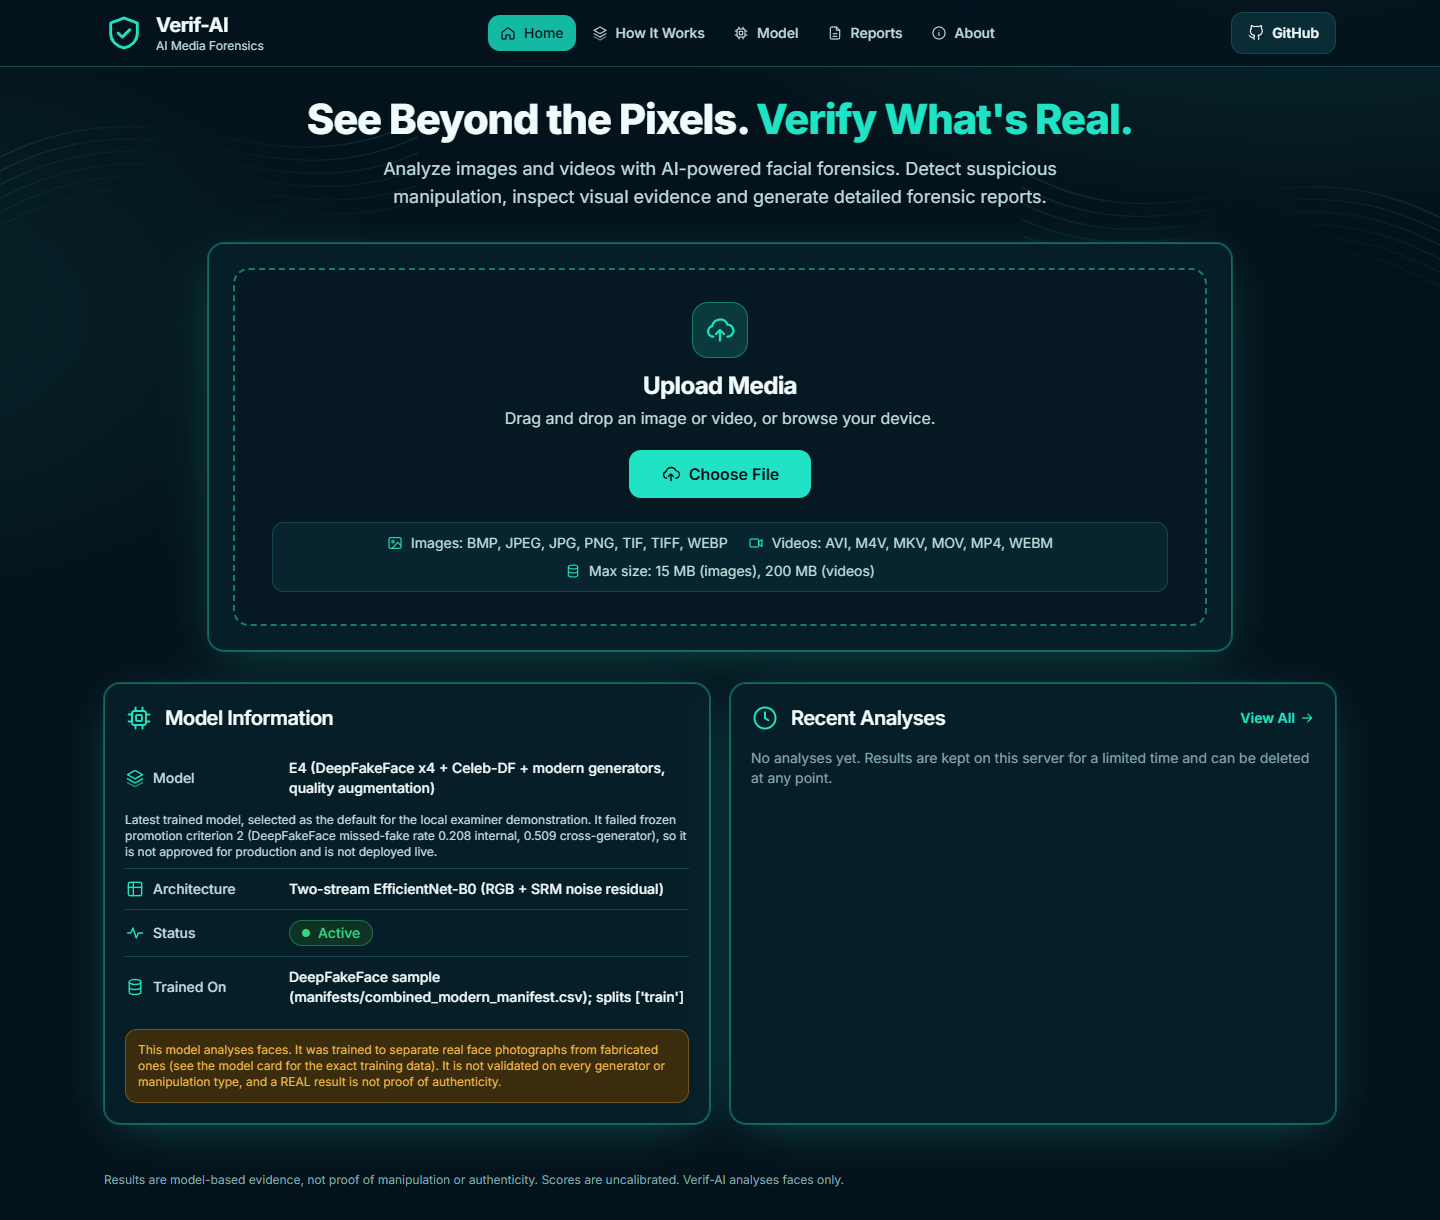
\includegraphics[width=0.6\linewidth]{screenshots/01_home.png}
\caption[Home page of the dashboard (current dark interface; screenshot taken from the running]{Home page of the dashboard (current dark interface; screenshot taken from the running application with an empty history).}
\label{fig:ui-home}
\end{figure}

\subsection{Deployment Architecture}
\label{sec:deploy-design}
The public demonstration separates a static frontend from a hosted API (Figure~\ref{fig:deploy}). The frontend is a build of the React
application served by Vercel; it reads the API address from a build-time environment variable. The API runs in a Docker container on
Render and answers browser requests only for the configured frontend origin (CORS). Results are written to the container's disk, which on the free
tier is not persistent. A paid instance with at least 2\,GB of memory and a disk would be required to run the full model with heat-maps and
durable results.

\begin{figure}[ht]
\centering
\begin{adjustbox}{max width=0.85\linewidth,center}
\begin{tikzpicture}[font=\footnotesize,
  n/.style={draw,rounded corners=3pt,minimum height=1.1cm,align=center,fill=white},
  arr/.style={-{Stealth[length=1.8mm]},thick}]
\node[n,fill=navy!8] (b) at (0,0) {Browser};
\node[n,fill=accent!10,minimum width=3.0cm] (v) at (4.3,0) {Vercel\\static React build};
\node[n,fill=accent!10,minimum width=3.4cm] (r) at (9.2,0) {Render web service\\(Docker, FastAPI + PyTorch)};
\node[n,fill=black!6,minimum width=3.4cm] (d) at (9.2,-2.0) {Instance disk\\(ephemeral on the free tier)};
\draw[arr,<->] (b)--node[above,font=\scriptsize]{page}(v);
\draw[arr,<->] (b.south)--++(0,-1.4)-|node[near start,below,font=\scriptsize]{API calls (CORS: Vercel origin only)}(r.south west);
\draw[arr] (r)--(d);
\end{tikzpicture}
\end{adjustbox}
\caption[Deployment architecture of the public demonstration]{Deployment architecture of the public demonstration. No uploaded media is sent to any service other than the API.}
\label{fig:deploy}
\end{figure}

\chapter{Implementation}
\label{ch:impl}

\section{Implementation and Engineering}
This chapter describes how the design of Chapter~\ref{ch:design} was realised: the environment, the module structure, the algorithms, the training
and evaluation tooling, the dashboard, the tests and the deployment. All code is in the project repository; key excerpts are listed in
Appendix~\ref{app:code}.

\subsection{Development Environment Setup}
The backend is a Python package (\code{backend/verifai}) installed from \code{requirements.txt}; training and development extras are
separate files. Configuration is read from environment variables or an optional \code{.env} file so that the same code runs locally, in
Docker and on a hosting service. The frontend (\code{frontend/}) is built with Vite and served either by the API process (single-container
mode) or by a static host. Typical commands are:

\begin{lstlisting}[language=bash,numbers=none,caption={Running the project locally.},label={lst:run}]
cd backend && python -m venv .venv && .venv\Scripts\activate
pip install -r requirements.txt
cd ../frontend && npm ci && npm run build
cd ../backend && set VERIFAI_FRONTEND_DIR=..\frontend\dist
python -m uvicorn verifai.api.app:app --host 127.0.0.1 --port 8000
\end{lstlisting}

\begin{table}[ht]
\centering
\caption{Core modules and file structure of the repository.}
\label{tab:modules}
\small
\begin{adjustbox}{max width=\linewidth,center}
\begin{tabular}{|p{4.4cm}|p{7.4cm}|}
\hline
\textbf{Module / path} & \textbf{Responsibility} \\ \hline
\code{verifai/config.py} & Settings from environment variables; default model order; limits \\ \hline
\code{verifai/model.py} & \texttt{SRMLayer}, \texttt{TwoStreamNet}, safe checkpoint loading, thread-safe prediction \\ \hline
\code{verifai/preprocess.py} & JPEG round-trip and ImageNet normalisation shared by training and inference \\ \hline
\code{verifai/faces.py} & MTCNN detection with confidence and size filters; box overlap for tracking \\ \hline
\code{verifai/registry.py} & Model registry: default / alternative / rollback roles, per-analysis selection, model identification \\ \hline
\code{verifai/scoring.py} & Labels, INCONCLUSIVE band, decisiveness, aggregation, temporal statistics, suspicious segments \\ \hline
\code{verifai/image_pipeline.py}, \code{video_pipeline.py} & Image and video analysis; evidence artifacts \\ \hline
\code{verifai/explain.py} & Grad-CAM on the RGB stream's last block \\ \hline
\code{verifai/report.py} & PDF forensic report \\ \hline
\code{verifai/store.py}, \code{engine.py} & Result storage, retention, background jobs, cancellation \\ \hline
\code{verifai/api/app.py} & FastAPI application, upload validation, routes, CORS \\ \hline
\code{training/} & Data preparation and validation, training, evaluation, degradations, stream ablation, quality bins, acceptance gate, modern-generator data \\ \hline
\code{frontend/src/} & Pages, result viewers, upload card, history, API client, tests \\ \hline
\code{kaggle/} & Builders for the private GPU notebooks \\ \hline
\code{docs/} & Architecture, evaluation, dataset, API, guides and experiment records \\ \hline
\end{tabular}
\end{adjustbox}
\end{table}

\subsection{Algorithm Specifications}
The operational logic is governed by three procedures. They make explicit the order of preprocessing and the way scores are aggregated.

\begin{algorithm}[ht]
\caption{Image analysis}
\label{alg:image}
\begin{algorithmic}[1]
\Require image file $I$, settings $S$, model $M$
\Ensure label and score for $I$, per-face results, evidence images
\State $rgb \gets \textsc{DecodeAndValidate}(I)$ \Comment{format, size, pixel limits}
\State $faces \gets \textsc{DetectFaces}(rgb)$ \Comment{MTCNN; keep conf $\ge0.90$, side $\ge32$\,px; at most 10}
\If{$faces=\emptyset$} \State \Return INCONCLUSIVE \Comment{no usable face is a result, not an error} \EndIf
\State $X \gets \textsc{Normalise}(\textsc{JpegRoundTrip}_{q=95}(\textsc{Crop}_{224}(faces)))$
\State $p \gets M(X)$ \Comment{raw sigmoid score per face}
\State $maps \gets \textsc{GradCAM}(M.\text{rgb\_stream},X)$ \Comment{skipped if unavailable}
\State $p_{img} \gets \max_i p_i$; \; $label \gets \textsc{Classify}(p_{img},\text{margin}=0.15)$
\State store annotated image, face crops, heat-maps; \Return $(label,p_{img})$
\end{algorithmic}
\end{algorithm}

\begin{algorithm}[ht]
\caption{Video analysis (background job)}
\label{alg:video}
\begin{algorithmic}[1]
\Require video file $V$, sampling rate $\approx2$\,fps, frame cap $64$
\Ensure verdict, tracks, suspicious ranges, evidence frames
\State $frames \gets \textsc{SampleFrames}(V)$; skip corrupt frames
\For{each frame $f$}
  \State $faces_f \gets \textsc{DetectFaces}(f)$; assign each face to a track by box overlap
\EndFor
\State score all face crops in batches; $s_f \gets \max$ face score in frame $f$
\State for every track with $\ge3$ observations: $s_{track} \gets \operatorname{median}$ of its scores
\State $p_{video} \gets \max_{track} s_{track}$ \Comment{pooled fallback when no track is long enough}
\State $ranges \gets$ maximal runs of consecutive frames with $s_f>0.5$
\State $E \gets$ six frames with highest $s_f$; store frame with boxes and Grad-CAM of its top face
\State \Return $(\textsc{Classify}(p_{video}),\ tracks,\ ranges,\ E)$
\end{algorithmic}
\end{algorithm}

\begin{algorithm}[ht]
\caption{Selecting what the frame viewer shows}
\label{alg:viewer}
\begin{algorithmic}[1]
\Require selected frame index $i$, analysed frames $F$, stored evidence $E$ (frame image, optional heat-map)
\State $e \gets E[i]$ if present
\If{$e$ exists}
  \State show the stored frame (with face boxes); show $e$.heatmap if it exists, else say ``not generated''
\Else
  \State say ``no frame image or heat-map was stored for this timestamp''; offer the nearest stored frame \Comment{nothing is approximated}
\EndIf
\State selecting a timestamp range $r$: choose the stored evidence frame with the highest score inside $r$, else the highest-scoring analysed frame
\end{algorithmic}
\end{algorithm}

\subsection{Module-wise Implementation Breakdown}
\textbf{Face localisation and normalisation.} Detection uses the pre-trained MTCNN of \citep{zhang2016mtcnn} through the
\texttt{facenet-pytorch} package. Detection runs on a downscaled copy for speed; boxes are scaled back and crops are cut from the original
image. The same detector produced all training crops.

\textbf{Model loading.} Checkpoints are loaded with weights-only deserialisation and strict key matching, so a mismatching file raises an error instead
of silently loading partial weights. Both the original prototype's raw state dictionaries and the new files with metadata are accepted. The
SHA-256 of the checkpoint is computed at load time and recorded in every result.

\textbf{Model registry.} The registry knows E4, Model 4 and v2. The server loads one default model at start-up (E4 locally; the hosted image pins v2); another model is loaded on first use and at most one such model stays in memory. \code{GET /api/models} lists the models with their roles, the analysis endpoints accept a \code{model} field, and every result, dashboard chip and PDF report records the model name, role, status note and checkpoint hash.

\textbf{Scoring and aggregation.} Labels use the fixed 0.5 threshold and the $\pm0.15$ reporting band. Aggregation methods (mean, median,
weighted mean, suspicious fraction) are implemented; the median is used. Temporal statistics and suspicious ranges are pure functions and are unit tested.

\textbf{Grad-CAM.} The heat-map is generated by the \texttt{grad-cam} package on the last block of the RGB stream. It needs gradients, so it runs
with autograd enabled under the model lock; it also needs extra memory, which matters on small hosts (Section~\ref{sec:deploy-impl}).

\textbf{PDF report.} The report is built with ReportLab from the stored result and evidence images. It contains the verdict banner, the
sentence that scores are not calibrated, analysis details (file hash, model, checkpoint hash, device, threshold), detected faces and
heat-maps, video tables where applicable and the limitations (Figure~\ref{fig:pdf}).

\textbf{Jobs and storage.} A single worker thread pool runs video jobs; a lock serialises model calls. On start-up interrupted jobs are
marked as failed, and a periodic clean-up removes results older than the retention time.

\begin{figure}[ht]
\centering
\begin{subfigure}[t]{0.47\linewidth}\centering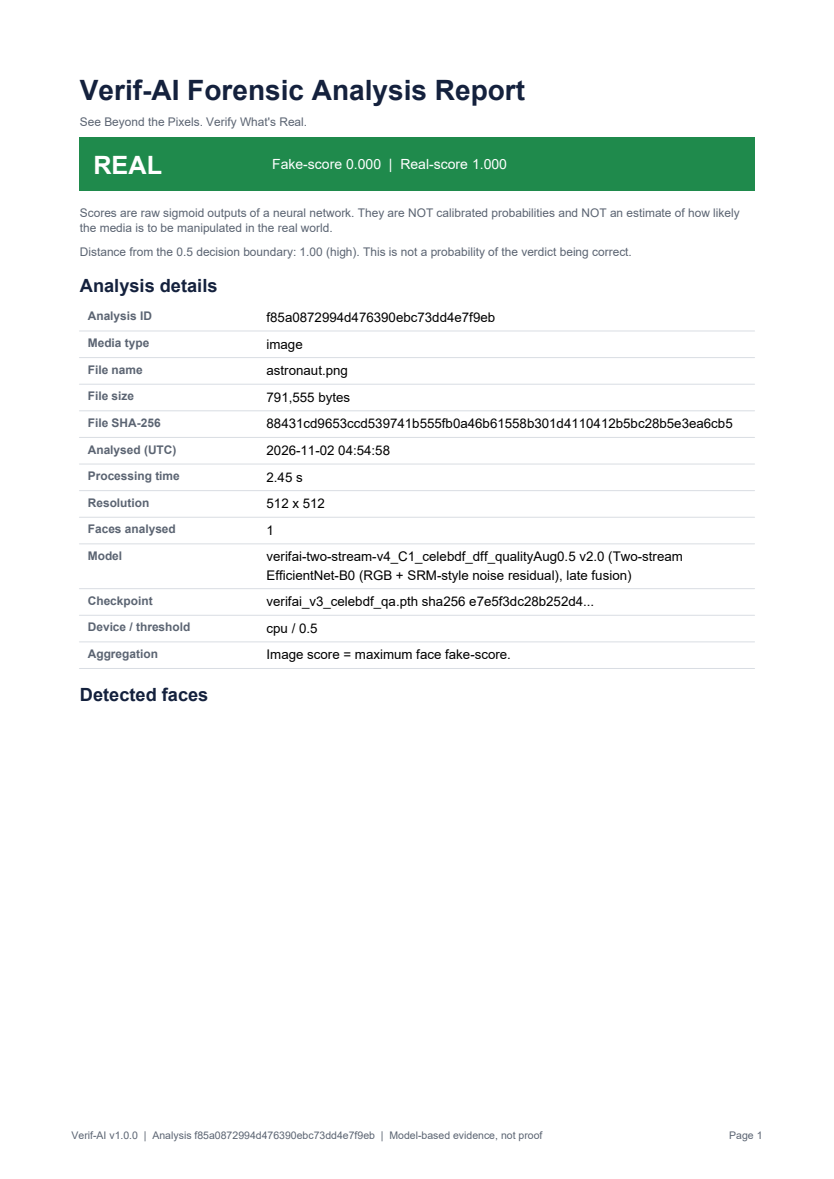
\includegraphics[width=\linewidth,height=1.4137\linewidth]{screenshots/17_pdf_report_p1.png}\caption{Page 1}\end{subfigure}\hfill
\begin{subfigure}[t]{0.47\linewidth}\centering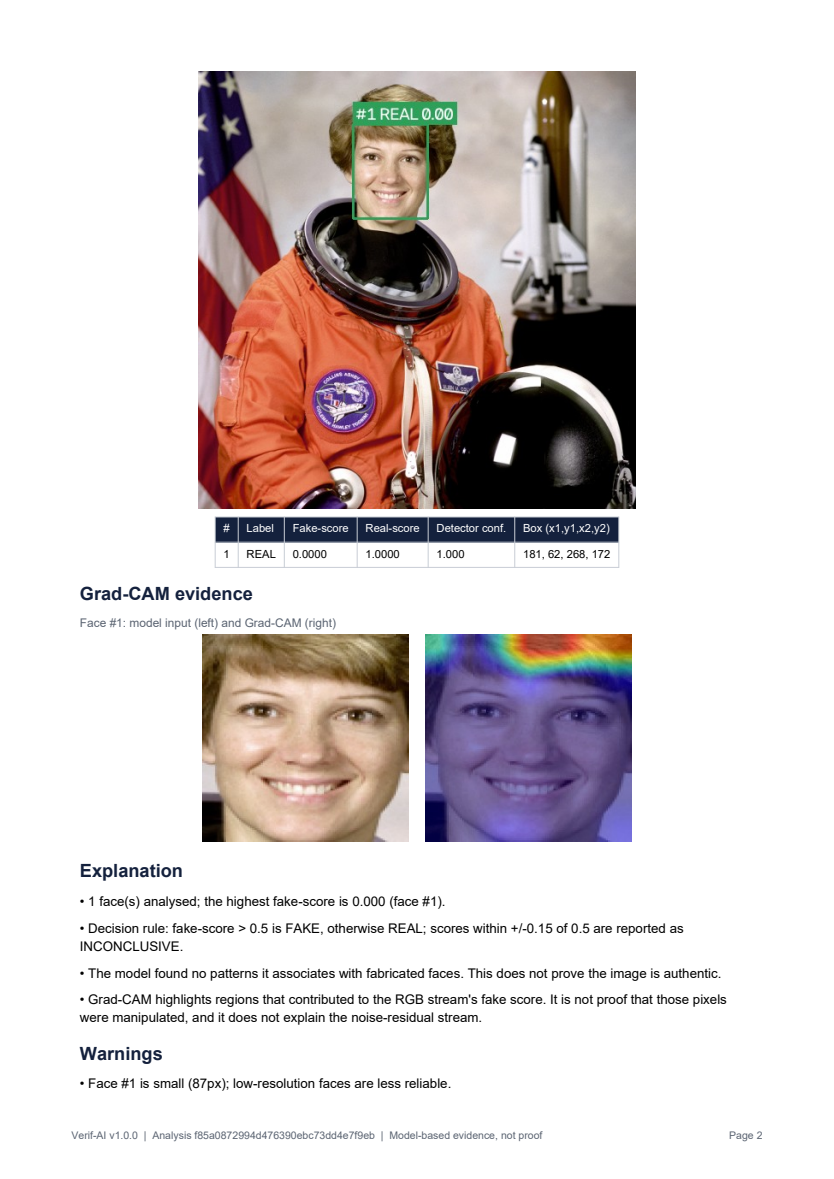
\includegraphics[width=\linewidth,height=1.4137\linewidth]{screenshots/17_pdf_report_p2.png}\caption{Page 2}\end{subfigure}
\caption[Pages 1 and 2 of a PDF forensic report generated by the application for a public test image]{Pages 1 and 2 of a PDF forensic report generated by the application for a public test image. The report records the verdict, the
uncalibrated-score statement, the file and checkpoint hashes and the detected face. (In this version the ``Detected faces'' heading is
separated from its image by a page break, a minor layout flaw.)}
\label{fig:pdf}
\end{figure}

\subsection{Training and Evaluation Implementation}
\textbf{Data preparation.} The DeepFakeFace subset was sampled with one fake counterpart per real image, cropped with the production
detector and split by \emph{identity and pair} so that no person appears in two splits; exact and perceptual duplicates were removed and the
split disjointness was verified by a validation script before training. Celeb-DF videos were split by identity and fakes that cross splits
were dropped. For experiment E3 the splits are file-disjoint and near-duplicates of training crops are removed from validation and test with a
64-bit difference hash (Hamming distance $\le3$).

\textbf{Training.} All models use AdamW \citep{loshchilov2019adamw} with learning rate $10^{-4}$, batch size 32, binary cross-entropy with logits
(positive-class weight set from the training class counts: 1.02 for the DeepFakeFace runs, 0.82 in E4), a learning-rate schedule that reduces on plateau, gradient clipping at 5, at most 12--15 epochs and early stopping with patience 4.
The best epoch is chosen on a \emph{validation} metric only. For the production model it is the validation ROC-AUC; for later experiments with degraded inputs it
is the mean of the clean and degraded validation ROC-AUC. Quality augmentation randomly applies blur, down-up resampling, JPEG compression, noise or low-light degradation.
Training ran in private Kaggle notebooks on a Tesla T4; only checkpoints and metrics were exported from notebooks that used third-party data.

\textbf{Evaluation tooling.} The evaluation script reports accuracy, precision, recall, F1, ROC-AUC, PR-AUC, confusion matrices and error rates
with grouped-bootstrap intervals, per generator and per split, at the fixed threshold, optionally under class-blind degradations; further
tools measure image sharpness bins, stream-level behaviour, an acceptance gate and video-level metrics.

\subsection{Frontend Implementation}
The dashboard is a React/TypeScript single-page application with hash routes, so a refresh or a deep link works on any static host. The
upload card validates the file type and size, detects images versus videos from the extension, shows a preview and calls the image or the video endpoint.
The result page is assembled only from fields of the API response; nothing is mocked or hard-coded.

\textbf{Heat-map viewer for images.} For each detected face the viewer shows the original face crop and the Grad-CAM image side by side, or
one of them alone, or an \emph{overlay} that blends the Grad-CAM image over the crop with an adjustable strength (Figure~\ref{fig:viewer}). Both
images are artifacts produced by the server; the interface does not compute or approximate a heat-map. If several faces are detected a selector
chooses which face is shown, and each face's verdict, score and detector confidence are displayed with it.

\begin{figure}[ht]
\centering
\begin{subfigure}[t]{0.47\linewidth}\centering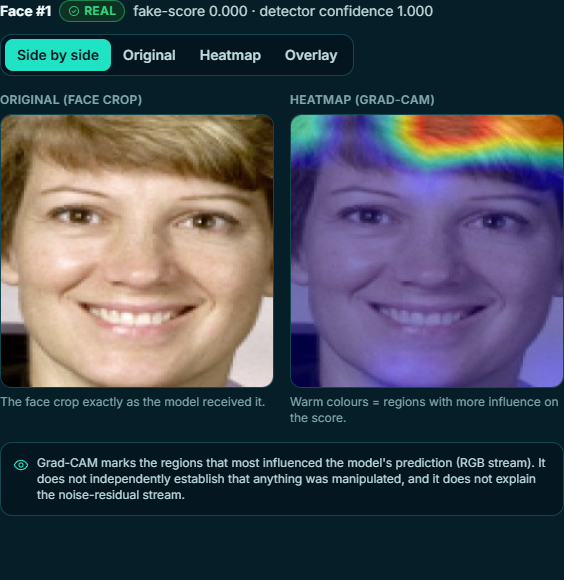
\includegraphics[width=\linewidth,height=1.0284\linewidth]{screenshots/pair_06_side_by_side.png}\caption{Side by side}\end{subfigure}\hfill
\begin{subfigure}[t]{0.47\linewidth}\centering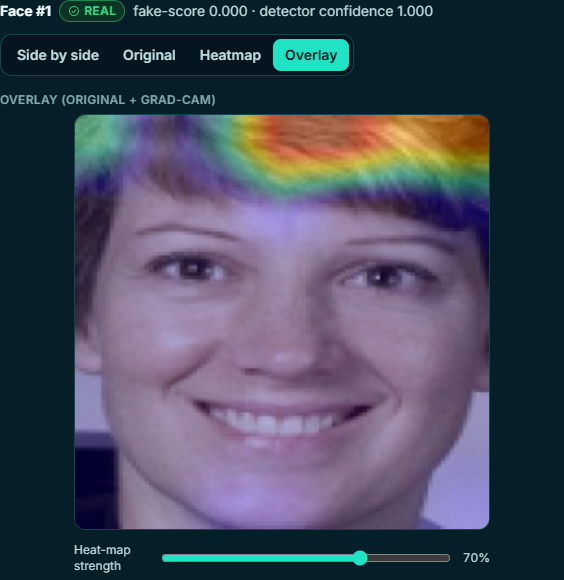
\includegraphics[width=\linewidth,height=1.0284\linewidth]{screenshots/pair_06d_overlay.png}\caption{Overlay (70\% strength)}\end{subfigure}
\caption[Heat-map viewer for an image result (public test image)]{Heat-map viewer for an image result (public test image). The viewer also offers Original-only and Heatmap-only views. The text
under the viewer states that Grad-CAM marks regions that influenced the model and does not establish manipulation.}
\label{fig:viewer}
\end{figure}

\textbf{Frame viewer for videos.} The timeline plots one dot per analysed frame; a dot is selectable. The selected frame's stored
image and heat-map come from the same evidence entry, so they cannot drift apart. Frames without stored evidence show an explicit notice and a
link to the nearest stored frame (Figure~\ref{fig:frames}). Selecting a suspicious time range jumps to the highest-scoring frame in it. The overlay
mode is disabled for video because the server stores the heat-map of the face crop but not its exact position in the frame, and a registered
overlay would be an approximation.

\begin{figure}[ht]
\centering
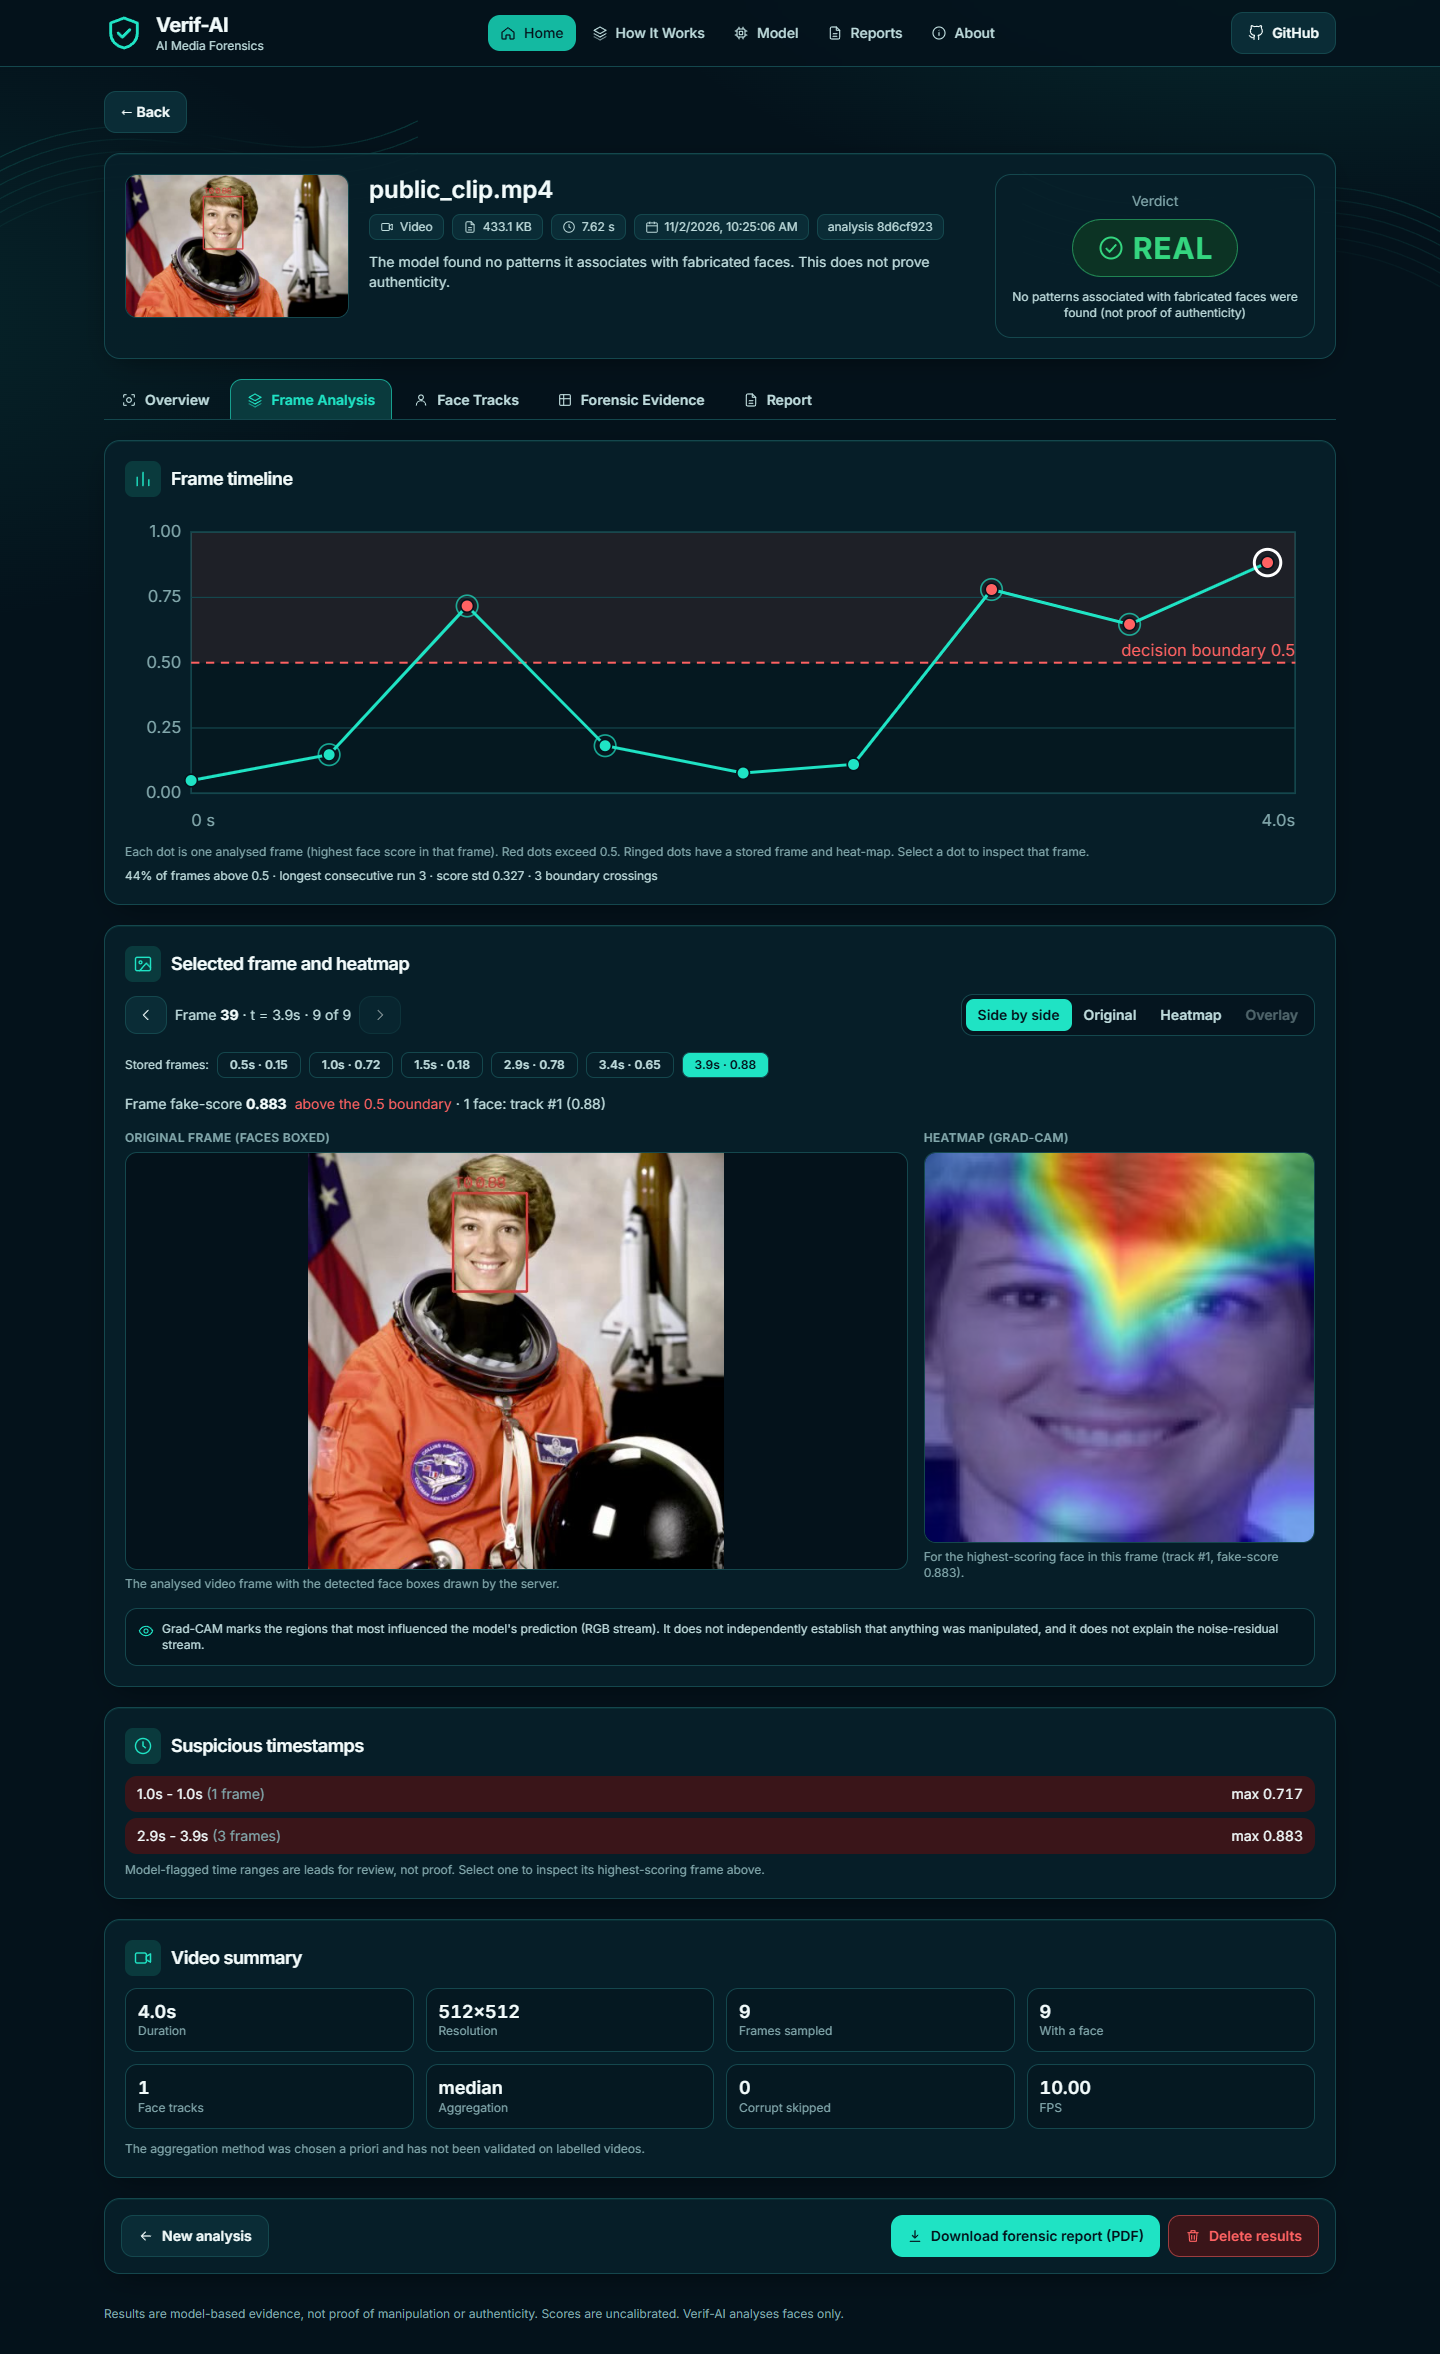
\includegraphics[width=0.96\linewidth,height=0.42\textheight,keepaspectratio]{screenshots/11_video_frame_analysis.png}
\caption[Frame Analysis tab for a video (a synthetic clip made from the public test image): the]{Frame Analysis tab for a video (a synthetic clip made from the public test image): the clickable timeline with the 0.5 decision
boundary, the selected frame with the face boxes and its Grad-CAM, and the stored-frame shortcuts.}
\label{fig:frames}
\end{figure}

\begin{figure}[ht]
\centering
\begin{subfigure}[t]{0.9\linewidth}\centering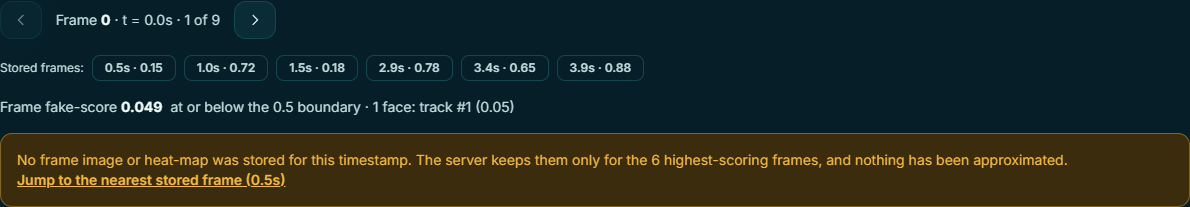
\includegraphics[width=\linewidth,height=0.17395\linewidth]{screenshots/pair_12_not_stored.png}\caption{Frame without stored evidence}\end{subfigure}\\[6pt]
\begin{subfigure}[t]{0.9\linewidth}\centering
\includegraphics[width=\linewidth,height=0.17395\linewidth]{screenshots/pair_13_face_tracks.png}\caption{Face Tracks tab (the card shown on the Face Tracks tab)}\end{subfigure}
\caption[Honest unavailability and face tracks]{Honest unavailability and face tracks. (a) The server keeps frames and heat-maps only for the six highest-scoring frames; other
frames say so. (b) Tracks with frame counts, time span, median score and the share of frames above 0.5.}
\label{fig:notstored}
\end{figure}

\begin{figure}[ht]
\centering
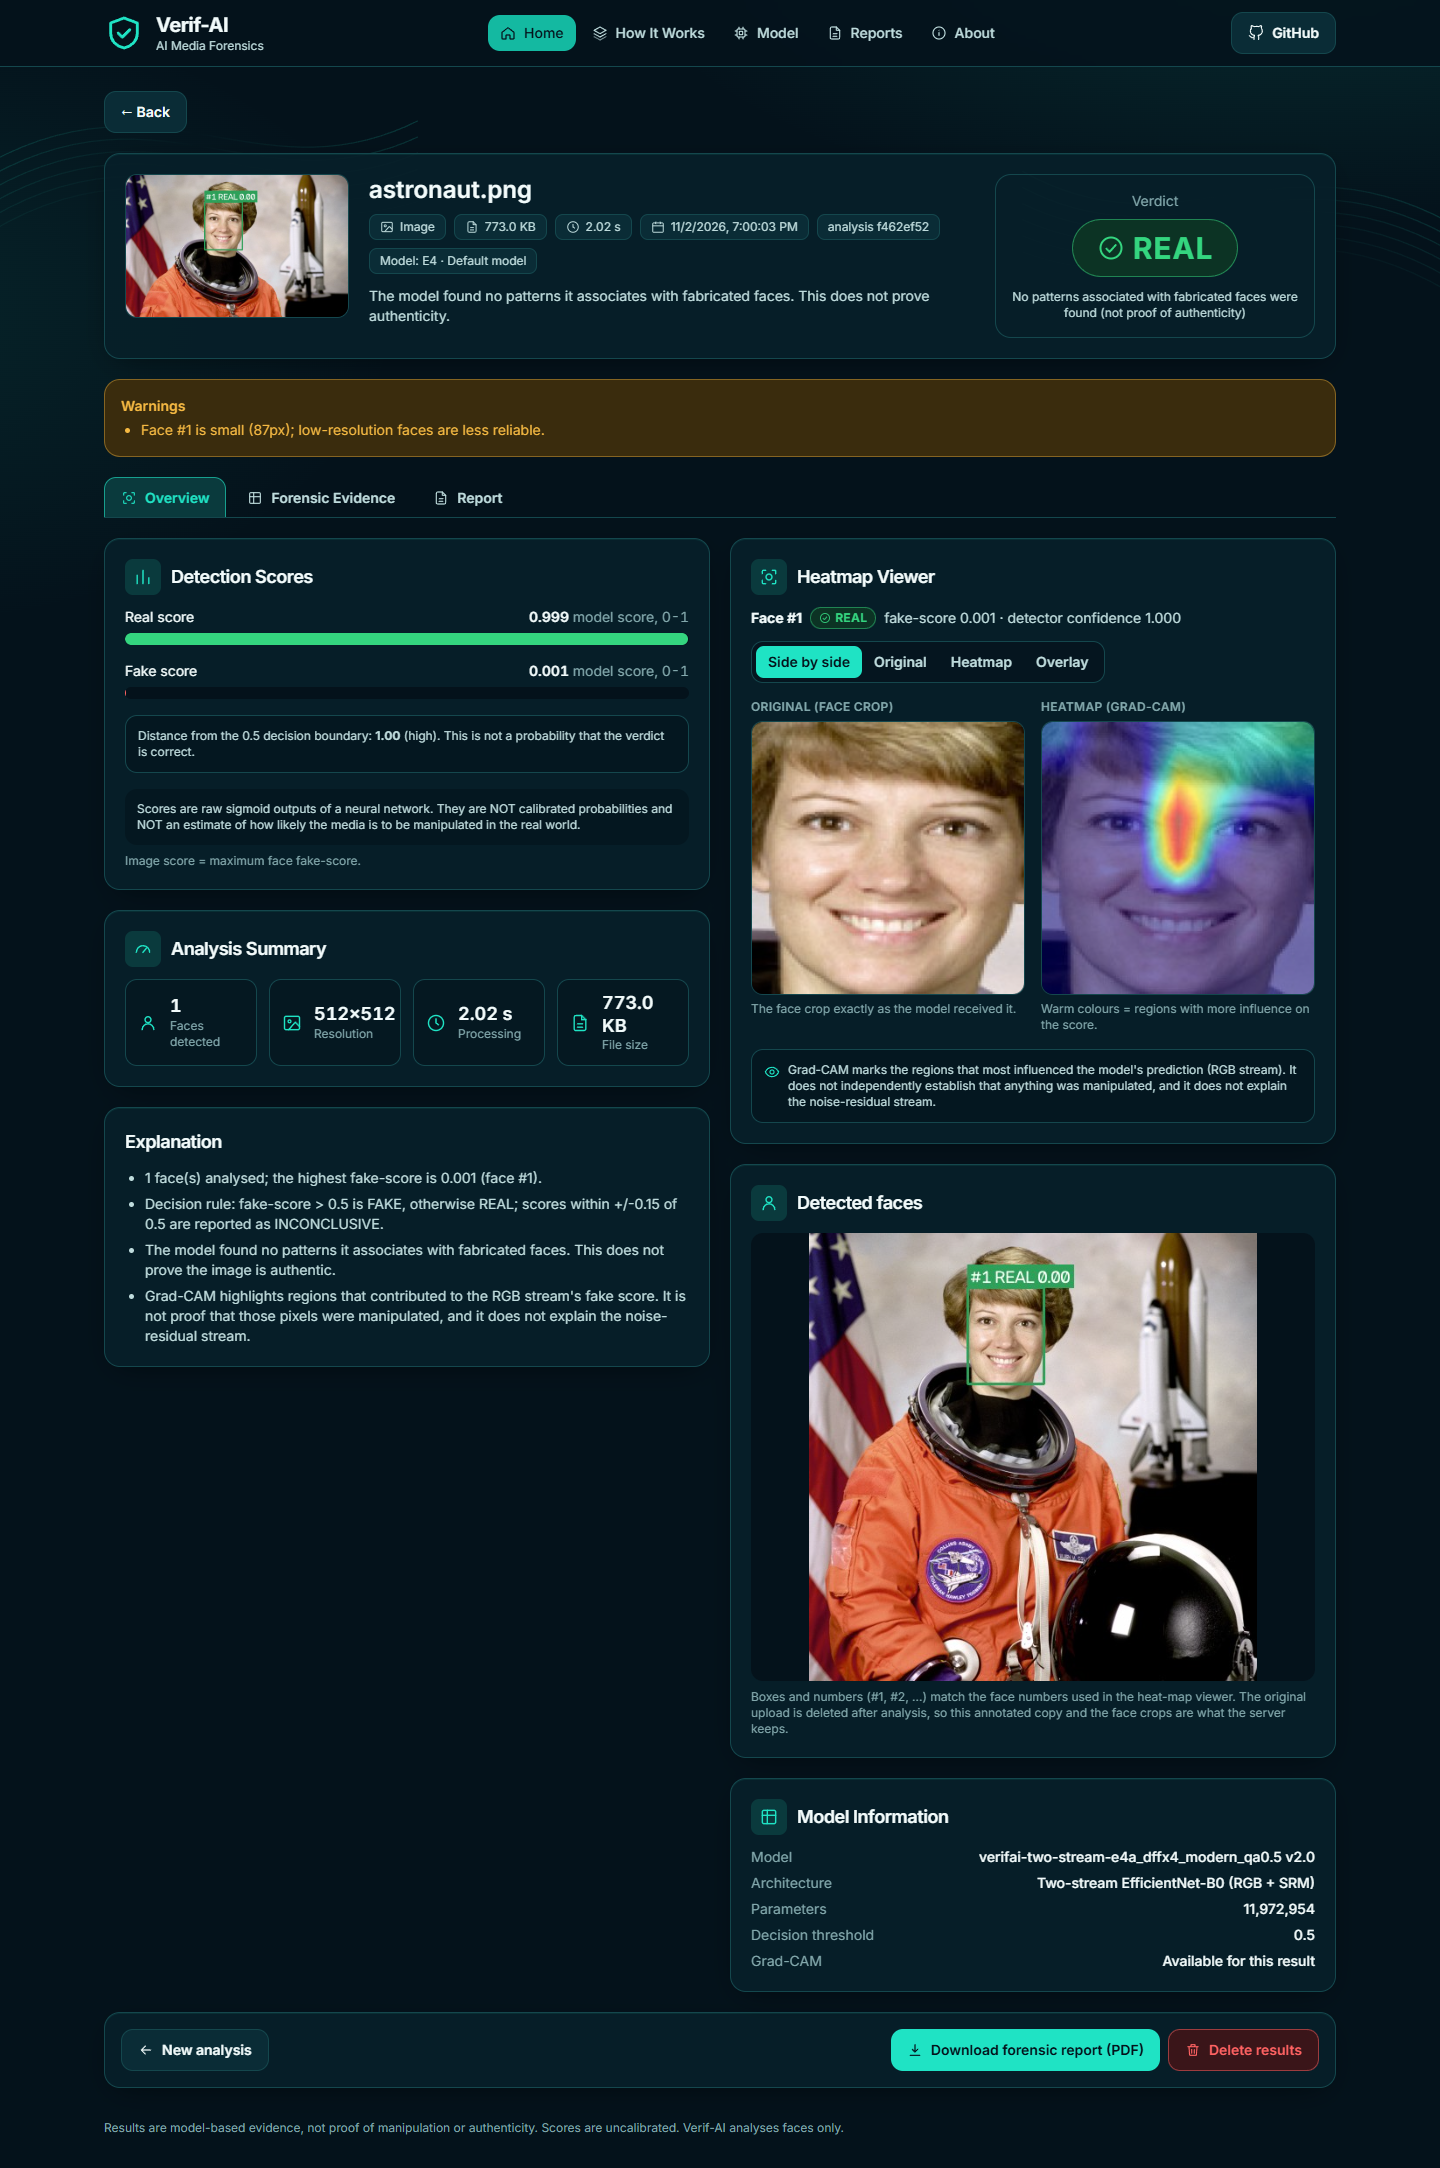
\includegraphics[width=0.96\linewidth,height=0.42\textheight,keepaspectratio]{screenshots/05_image_result_overview.png}
\caption[Overview tab of an image result: verdict, model score labelled as uncalibrated, analysis summary, the heat-map viewer and the detected faces with bounding boxes]{Overview tab of an image result: verdict, model score labelled as uncalibrated, analysis summary, the heat-map viewer and the detected
faces with bounding boxes. The ``Trained On'' text in the model panel (Figure~\ref{fig:ui-home}) is the checkpoint's own metadata, which
understates the data used for this model (Section~\ref{sec:limits}).}
\label{fig:result}
\end{figure}

\textbf{History and deletion.} Because a public API should not list other visitors' analyses, the dashboard stores the identifiers of the
analyses created in that browser and asks the server for each one; deleted or expired identifiers are dropped. Deleting a result removes
the server-side folder and the local entry.

\subsection{Testing and Verification}
Verification was automated wherever possible. The backend suite covers model loading, data validation, scoring and tracking, the image and
video pipelines, the API, the PDF report, training smoke tests and the research tooling; at the time of writing 152 tests passed and 7 were
skipped because they need a test video, a GPU or private media (the skips are environment-gated and were not hidden). The frontend has 63
unit and component tests (including the viewer modes, frame synchronisation and the unavailable states) and 9 Playwright end-to-end tests that
drive a real Chrome browser: unified upload, image and video analysis, heat-map modes, timeline selection, PDF download, deletion, rejected
files, navigation and refresh, console errors and layouts from 1440 to 320 pixels wide. The end-to-end suite was run against the local server, against a separate
frontend origin and against the public deployment.

\subsection{Deployment Implementation}
\label{sec:deploy-impl}
\textbf{Frontend.} The frontend is deployed on Vercel as a static build; \code{vercel.json} fixes the build command and output directory and adds
security headers, and the API address is the build-time variable \code{VITE_API_BASE_URL}. Direct navigation and a refresh were verified on
the public URL.

\textbf{Backend.} The API runs in a Docker container on Render's free tier with CORS limited to the Vercel origin. The memory needed by the
backend was measured on the development laptop (Table~\ref{tab:memory}).

\begin{table}[ht]
\centering
\caption[Backend memory (process working set, MB) measured on the development laptop for different]{Backend memory (process working set, MB) measured on the development laptop for different configurations.}
\label{tab:memory}
\small
\begin{adjustbox}{max width=\linewidth,center}
\begin{tabular}{|p{5.6cm}|c|c|c|}
\hline
\textbf{Configuration} & \textbf{Idle} & \textbf{Image peak} & \textbf{Video peak} \\ \hline
Default (Grad-CAM on, batch 16) & 491 & 776 & over 818 \\ \hline
Grad-CAM on, batch 2, one thread & 488 & 672 & 1473 \\ \hline
Grad-CAM off, batch 2, one thread & 488 & 510 & 576 \\ \hline
\end{tabular}
\end{adjustbox}
\end{table}

A 512\,MB instance cannot run the default configuration: the first analysis on the free tier returned HTTP 502 (the process was killed for lack of memory). The
public instance therefore runs in a restricted ``lite'' mode with Grad-CAM disabled, small batches, a single thread and small upload limits; the
interface reports that heat-maps are unavailable instead of failing. It serves the model checkpoint contained in the repository (v2) because
the newer checkpoint is not stored in Git and the free tier has no persistent disk. Results disappear when the instance restarts and the first
request after an idle period takes about a minute. \textbf{This deployment is a restricted demonstration, not a production system;} full
functionality needs at least 2\,GB of memory and a disk, authentication and rate limiting.

\subsection{Engineering Challenges and Optimisations}
\begin{itemize}
\item \textbf{Identical preprocessing.} Training crops had been stored as JPEG, so inference reproduces the JPEG round-trip; without it the scores
differ from the evaluated ones.
\item \textbf{Leakage control.} Identity-disjoint splits and duplicate removal were implemented before training; later experiments add near-duplicate
removal across training, validation and test (179 validation and 373 test crops were removed in E3).
\item \textbf{Memory.} The memory profile above led to configurable batch sizes, optional Grad-CAM and the lite mode.
\item \textbf{Privacy.} Deleting uploads in all code paths, expiring results and removing the public history list required changes in
both backend and frontend.
\item \textbf{Third-party data.} Notebooks that use third-party images export only checkpoints and metrics; a failed run's output can contain
working files, so logs were read through the API without downloading outputs.
\end{itemize}

\chapter{Results and Discussion}
\label{ch:results}

\section{Results, Evaluation and Discussion}
This chapter presents the experiments in the order in which they were carried out, because each one explains the next: the production
model and its measured performance, a failure on genuine video, the diagnosis of that failure as an image-quality shortcut, an acceptance
gate, a retraining that fixed the video failure at a cost, and an experiment with modern generators. Every number comes from a saved result
file of the repository; the limits of each number are stated next to it.

\subsection{Experimental Setup and Dataset Partitioning}
\textbf{DeepFakeFace (DFF).} A sample of the dataset \citep{song2023dff} was used. The real images are IMDB-WIKI photographs
\citep{rothe2018imdbwiki}; for each real image one fake counterpart is generated by inpainting, face swapping (``insight'') or a text-to-image
model (``text2img''). Splits are identity- and pair-disjoint after duplicate removal (Table~\ref{tab:dffsplits}). The text-to-image fakes occur
only in the cross-generator test split, so that split measures behaviour on an \emph{unseen generator}.

\begin{table}[ht]
\centering
\caption{DeepFakeFace splits used for the production model (face crops).}
\label{tab:dffsplits}
\small
\begin{adjustbox}{max width=\linewidth,center}
\begin{tabular}{|l|p{3.4cm}|c|p{3.4cm}|}
\hline
\textbf{Split} & \textbf{Role} & \textbf{n (real / fake)} & \textbf{Fake generators} \\ \hline
train & fitting & 2{,}315 (1{,}170 / 1{,}145) & inpainting, insight \\ \hline
val & model selection & 471 (239 / 232) & inpainting, insight \\ \hline
test\_internal & unseen identities, seen generators & 575 (292 / 283) & inpainting, insight \\ \hline
test\_crossgen & unseen identities and unseen generator & 568 (281 / 287) & text2img \\ \hline
\end{tabular}
\end{adjustbox}
\end{table}

\textbf{Celeb-DF v2.} Videos \citep{li2020celebdf} were split by identity into training, validation and held-out test identities (nine test identities,
147 videos: 91 real and 56 fake); fakes whose source and target identities fall in different splits were dropped. Frames were sampled from
each video, cropped with the production detector and stored as JPEG. Test results are reported at frame level and at video level.

\textbf{Experiment E3 data.} Modern-generator data were added from FFHQ real faces \citep{karras2019stylegan}, SFHQ synthetic faces
\citep{sfhq2022} and the fake side of the DeepDetect-2025 collection (Table~\ref{tab:e3data}). The datasets were reviewed for provenance and
shortcuts before use (Appendix~\ref{app:datasets}); two candidate datasets were excluded.

\begin{table}[ht]
\centering
\caption[Composition of the experiment E3 manifest after face detection and near-duplicate removal]{Composition of the experiment E3 manifest after face detection and near-duplicate removal (crops).}
\label{tab:e3data}
\small
\begin{adjustbox}{max width=\linewidth,center}
\begin{tabular}{|p{3.3cm}|c|c|c|p{4.0cm}|}
\hline
\textbf{Source (label)} & \textbf{Train} & \textbf{Val.} & \textbf{modern\_test} & \textbf{Notes} \\ \hline
FFHQ (real) & 7{,}996 & 966 & 1{,}447 & file-disjoint, seed 42 \\ \hline
SFHQ (fake) & 3{,}000 & 473 & 677 & StyleGAN-generated \\ \hline
DeepDetect fake & 8{,}997 & 880 & 2{,}202 & modern generators; no per-image generator label \\ \hline
DeepFakeFace + Celeb-DF & as for Model 4 & as before & separate tests & original splits unchanged \\ \hline
\end{tabular}
\end{adjustbox}
\end{table}

\subsection{Performance Evaluation Methodology}
\textbf{Metrics.} With ``fake'' as the positive class the report uses accuracy, precision, recall, F1, the area under the ROC curve (ROC-AUC), the
false-positive rate (FPR: genuine faces called fake) and the false-negative rate (FNR: fakes called genuine), together with confusion matrices.
Intervals are Wilson 95\% intervals \citep{wilson1927} for rates and grouped-bootstrap intervals \citep{efron1993bootstrap} for the other metrics.

\textbf{Rules fixed in advance.} (i) The decision threshold is 0.5 and is never tuned. (ii) Model selection uses \emph{validation} data
only; test data are never used for selection or for thresholds. (iii) Results on held-out identities with seen generators (\emph{internal}) are always
reported separately from results on an unseen generator (\emph{cross-generator}). (iv) Celeb-DF results are \emph{within-dataset} evidence:
the held-out identities share the face-swap method and the footage type of the training videos, so they say nothing about other
manipulation methods. (v) Scores are raw sigmoid outputs, not probabilities.

\subsection{Results for the Production Model v2 (DeepFakeFace)}
The production model v2 was chosen among three training configurations by validation ROC-AUC alone (ImageNet initialisation, 9th epoch,
validation ROC-AUC 0.948); its test numbers were never consulted for selection. Table~\ref{tab:v2} shows its results.

\begin{table}[ht]
\centering
\caption[Production model v2 on DeepFakeFace (threshold 0.5; fake is positive; intervals are 95\%]{Production model v2 on DeepFakeFace (threshold 0.5; fake is positive; intervals are 95\% grouped bootstrap).}
\label{tab:v2}
\small
\begin{adjustbox}{max width=\linewidth,center}
\begin{tabular}{|l|c|c|c|c|c|c|}
\hline
\textbf{Split} & \textbf{Acc} & \textbf{Prec} & \textbf{Recall} & \textbf{F1} & \textbf{ROC-AUC} & \textbf{FPR / FNR} \\ \hline
Validation (selection) & 0.877 & 0.843 & 0.922 & 0.881 & 0.948 (0.928--0.965) & 0.167 / 0.078 \\ \hline
Internal test & 0.875 (0.848--0.902) & 0.860 & 0.890 & 0.875 & 0.941 (0.921--0.960) & 0.140 / 0.110 \\ \hline
Cross-generator test & 0.746 (0.716--0.778) & 0.818 & 0.641 & 0.719 & 0.849 (0.818--0.879) & 0.146 / 0.359 \\ \hline
\end{tabular}
\end{adjustbox}
\end{table}

\begin{figure}[ht]
\centering
\begin{subfigure}[t]{0.47\linewidth}\centering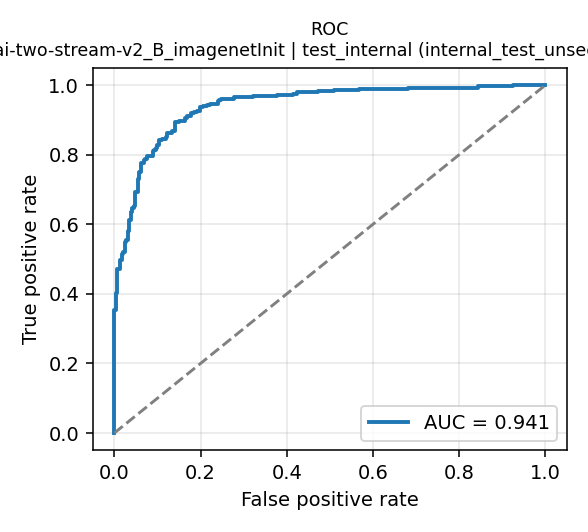
\includegraphics[width=\linewidth,height=0.9048\linewidth]{figures/v2_roc_test_internal.png}\caption{Internal test}\end{subfigure}\hfill
\begin{subfigure}[t]{0.47\linewidth}\centering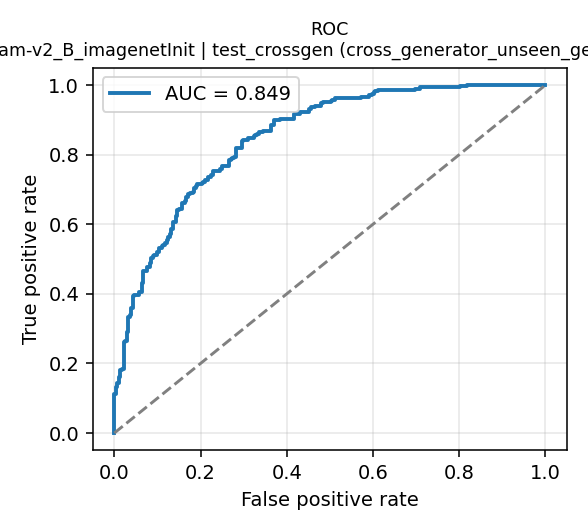
\includegraphics[width=\linewidth,height=0.9048\linewidth]{figures/v2_roc_test_crossgen.png}\caption{Cross-generator test}\end{subfigure}
\caption[ROC curves of v2 on the two held-out DeepFakeFace test splits (generated by the evaluation]{ROC curves of v2 on the two held-out DeepFakeFace test splits (generated by the evaluation script).}
\label{fig:v2roc}
\end{figure}

\begin{figure}[ht]
\centering
\begin{subfigure}[t]{0.47\linewidth}\centering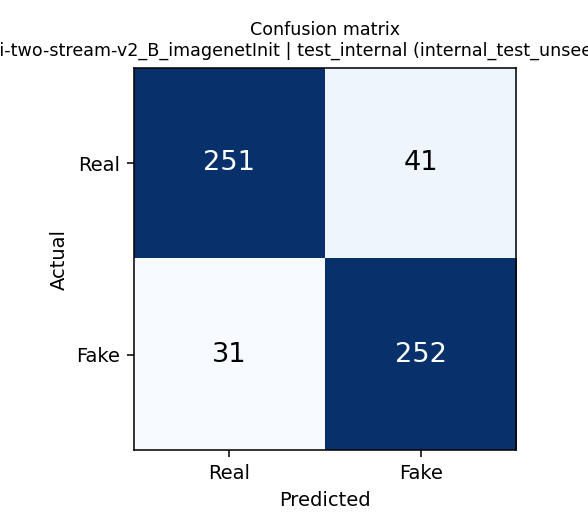
\includegraphics[width=\linewidth,height=0.9048\linewidth]{figures/v2_confusion_matrix_test_internal.png}\caption{Internal test}\end{subfigure}\hfill
\begin{subfigure}[t]{0.47\linewidth}\centering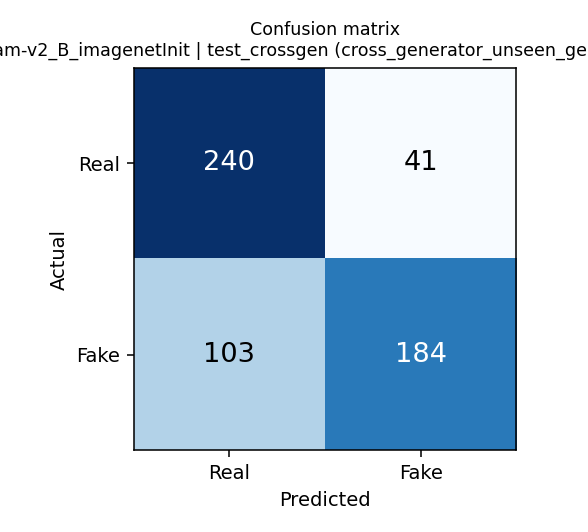
\includegraphics[width=\linewidth,height=0.9048\linewidth]{figures/v2_confusion_matrix_test_crossgen.png}\caption{Cross-generator test}\end{subfigure}
\caption[Confusion matrices of v2 at threshold 0.5]{Confusion matrices of v2 at threshold 0.5. On the unseen generator the model misses a much larger share of fakes (103 of 287).}
\label{fig:v2cm}
\end{figure}

On the internal split v2 detects inpainting fakes 91.5\% and face swaps 86.6\% of the time and accepts 85.9\% of real photographs. On the unseen
text-to-image generator the detection rate falls to 64.1\%. This gap between internal and cross-generator performance is the first
evidence that the measured accuracy depends on the generators seen during training, and \emph{the internal numbers must not be quoted as general accuracy}.
For comparison, the original prototype's checkpoint, evaluated on the same identity-disjoint data, performed at chance level; the very high accuracy
reported for the prototype could therefore not be reproduced under this protocol.

\subsection{A Failure on Genuine Video: the Four-Model Comparison}
When genuine video of a person was analysed with v2, the application sometimes reported FAKE with very high scores. To test this
systematically, four models were evaluated with identical code on the held-out Celeb-DF identities: Model~1 (production v2), Model~2 (DeepFakeFace only with
quality augmentation), Model~3 (DeepFakeFace plus Celeb-DF) and Model~4 (as Model 3 with quality augmentation). Table~\ref{tab:fourvideo} gives the video-level results.

\begin{table}[ht]
\centering
\caption[Video-level results on 147 held-out Celeb-DF videos (91 real, 56 fake), clean inputs, 95\%]{Video-level results on 147 held-out Celeb-DF videos (91 real, 56 fake), clean inputs, 95\% Wilson intervals.}
\label{tab:fourvideo}
\small
\begin{adjustbox}{max width=\linewidth,center}
\begin{tabular}{|l|c|c|c|}
\hline
\textbf{Model} & \textbf{Accuracy} & \textbf{FPR (real called fake)} & \textbf{FNR (fake called real)} \\ \hline
1 Production v2 & 0.483 (0.404--0.563) & 55/91 = 0.604 (0.502--0.699) & 21/56 = 0.375 (0.260--0.506) \\ \hline
2 DFF only + quality aug. & 0.578 (0.497--0.655) & 16/91 = 0.176 (0.111--0.267) & 46/56 = 0.821 (0.702--0.900) \\ \hline
3 DFF + Celeb-DF & 0.973 (0.932--0.989) & 4/91 = 0.044 (0.017--0.108) & 0/56 = 0.000 (0.000--0.064) \\ \hline
4 DFF + Celeb-DF + quality aug. & 0.980 (0.942--0.993) & 2/91 = 0.022 (0.006--0.077) & 1/56 = 0.018 (0.003--0.094) \\ \hline
\end{tabular}
\end{adjustbox}
\end{table}

The production model is at chance level on this video set (55 of 91 genuine videos called fake). Models trained on Celeb-DF frames reach
0.97--0.98 video accuracy, but this is \emph{within-dataset} evidence: the test identities share the face-swap method and the footage type of the training videos.
Adding Celeb-DF also had a cost on DeepFakeFace: Model 4's false-negative rate on the unseen generator rose from 0.359 (v2) to 0.634, and on the internal test from 0.110 to 0.201 (Table~\ref{tab:e3-frame}).

\subsection{Diagnosis: an Image-Quality Shortcut}
\label{sec:diag}
Experiment E1 measured whether image sharpness alone predicts the label (no model involved). In DeepFakeFace the fakes are softer than the real
photographs: the ROC-AUC of \emph{softness alone} as a classifier of FAKE is 0.712 (95\% CI 0.696--0.729) on the training split, 0.680 on the internal
test split and --- on the unseen generator --- \textbf{0.432}, i.e.\ the cue reverses. The share of fakes among crops rises from 26\% in the sharpest
bin to 85\% in the softest (Figure~\ref{fig:shortcut}). Celeb-DF frames are almost all very soft (about 94\% fall into the softest sharpness bin, against about 8\% of DeepFakeFace training crops), so a model trained on
DeepFakeFace alone has seen almost no soft real faces and learns ``soft face means fake'', which explains the false alarms on soft genuine video.
Stream-level analysis showed that the noise stream carries this dependence: the Spearman correlation between sharpness and the noise-stream score was $-0.36$
(real faces) and $-0.52$ (fake faces) for the production model on the DeepFakeFace internal test split, while the RGB stream's correlation was close to zero. On the
Celeb-DF validation faces the production model's noise stream alone called 98.7\% of the real faces fake (stage-0 diagnostics).

\begin{figure}[ht]
\centering
\begin{adjustbox}{max width=\linewidth,center}
\begin{tikzpicture}
\begin{axis}[width=0.92\linewidth,height=6.2cm,ybar,bar width=7pt,ymin=0,ymax=100,ylabel={Fake share of crops (\%)},
  symbolic x coords={{$<40$},{40--80},{80--160},{160--320},{$\ge320$}},xtick=data,xlabel={Sharpness bin (variance of Laplacian)},
  legend style={at={(0.5,1.02)},anchor=south,legend columns=3,font=\footnotesize},tick label style={font=\footnotesize},
  enlarge x limits=0.15,ymajorgrids]
\addplot[fill=navy!70] coordinates {({$<40$},85)({40--80},71)({80--160},56)({160--320},40)({$\ge320$},26)};
\addplot[fill=accent!70] coordinates {({$<40$},75)({40--80},71)({80--160},53)({160--320},39)({$\ge320$},30)};
\addplot[fill=orange!80] coordinates {({$<40$},22)({40--80},43)({80--160},44)({160--320},53)({$\ge320$},55)};
\legend{DFF train,DFF internal test,DFF cross-generator test}
\end{axis}
\end{tikzpicture}
\end{adjustbox}
\caption[Fake share per fixed sharpness bin in DeepFakeFace (values from the E1 diagnostic)]{Fake share per fixed sharpness bin in DeepFakeFace (values from the E1 diagnostic). In the training and internal splits softness predicts
``fake''; on the unseen generator the relation is reversed, which shows that sharpness is a dataset shortcut and not a manipulation cue.}
\label{fig:shortcut}
\end{figure}

\subsection{The Stage-0 Acceptance Gate}
Because overall accuracy hides this kind of failure, a per-quality-bin acceptance gate was designed and its thresholds were frozen in a
protocol document before any run. It checks that each stream separates the classes on its own (G1), that scores are not correlated with
sharpness within a class (G2), that error rates do not vary across quality bins (G3) and that the model separates the classes within bins (G4),
on validation data only, clean and with class-blind degradations. Synthetic controls validate the gate itself: a softness-only classifier
must fail it and a quality-independent scorer must not. All four models failed the gate (Table~\ref{tab:gate}); models 3 and 4 pass the
ungated screen (ROC-AUC $\ge0.90$ on both clean validation sets) yet fail the gate, which shows that the gate carries information that the aggregate metric does not.
The thresholds were chosen while reading E1 results that included test splits, so stage-0 cannot prove independence of its thresholds from the test data; this is stated as a limitation.

\begin{table}[ht]
\centering
\caption[Stage-0 gate results (validation data, clean and degraded sets; DFF = DeepFakeFace, CDF =]{Stage-0 gate results (validation data, clean and degraded sets; DFF = DeepFakeFace, CDF = Celeb-DF).}
\label{tab:gate}
\small
\begin{adjustbox}{max width=\linewidth,center}
\begin{tabular}{|l|c|p{6.0cm}|}
\hline
\textbf{Model} & \textbf{Passes ungated screen} & \textbf{Gate failures (set:check)} \\ \hline
1 Production v2 & no & 13 failures across DFF and CDF, clean and degraded \\ \hline
2 DFF only + quality aug. & no & 9 failures \\ \hline
3 DFF + Celeb-DF & yes & DFF-clean:G3; DFF-degraded:G1--G4; CDF-degraded:G2--G4 \\ \hline
4 DFF + Celeb-DF + quality aug. & yes & DFF-clean:G2; DFF-degraded:G1; CDF-degraded:G2 \\ \hline
\end{tabular}
\end{adjustbox}
\end{table}

\subsection{Experiment E3: Modern-Generator Training}
\label{sec:e3}
The protocol of E3 (data, leakage control, candidates, evaluation, promotion rule) was written \emph{before} training. Two candidates were
trained on the enlarged data with the Model-4 recipe: E3A with quality augmentation and E3B without. The choice between them used validation only
(E3A, validation selection score 0.980 against 0.939). Both were evaluated with Model 4 and v2 under the same protocol (Tables~\ref{tab:e3-frame}--\ref{tab:e3-mixed}).

\textbf{Reading the tables.} The ``Validation'' row is the \emph{combined} E3 validation split, which includes modern-generator and Celeb-DF crops
that Model 4 and v2 were never trained on; their low accuracy there reflects that mismatch and is not a regression. The E3 evaluation re-extracted the Celeb-DF crops, so
the Celeb-DF numbers differ slightly from the earlier four-model comparison (Model 4: video accuracy 0.980 in both; v2: 0.476 here against 0.483 there).

% generated by report/scripts/make_tables.py from docs/results/e3_modern/e3_selection.json
\begin{table}[ht]\centering\caption[Frame-level results, clean inputs, fixed threshold 0.5 (FPR: real called FAKE; FNR: fake called REAL; 95\% Wilson intervals)]{Frame-level results, clean inputs, fixed threshold 0.5 (FPR: real called FAKE; FNR: fake called REAL; 95\% Wilson intervals). Counts are real / fake crops.}\label{tab:e3-frame}\scriptsize\resizebox{\ifdim\width>\linewidth\linewidth\else\width\fi}{!}{\begin{tabular}{|l|l|c|c|c|c|c|}\hline
\textbf{Split} & \textbf{Model} & \textbf{n (R/F)} & \textbf{Acc} & \textbf{AUC} & \textbf{FPR} & \textbf{FNR} \\ \hline
Validation & E3A & 2045/2410 & 0.952 & 0.990 & 0.039 [0.03,0.05] & 0.056 [0.05,0.07] \\
 & E3B & 2045/2410 & 0.954 & 0.992 & 0.056 [0.05,0.07] & 0.037 [0.03,0.05] \\
 & Model 4 & 2045/2410 & 0.654 & 0.713 & 0.066 [0.06,0.08] & 0.583 [0.56,0.60] \\
 & v2 & 2045/2410 & 0.489 & 0.484 & 0.319 [0.30,0.34] & 0.675 [0.66,0.69] \\
\hline
DFF internal test & E3A & 292/283 & 0.833 & 0.916 & 0.106 [0.08,0.15] & 0.230 [0.18,0.28] \\
 & E3B & 292/283 & 0.861 & 0.939 & 0.130 [0.10,0.17] & 0.148 [0.11,0.19] \\
 & Model 4 & 292/283 & 0.835 & 0.921 & 0.130 [0.10,0.17] & 0.201 [0.16,0.25] \\
 & v2 & 292/283 & 0.875 & 0.941 & 0.140 [0.11,0.18] & 0.110 [0.08,0.15] \\
\hline
DFF cross-generator test & E3A & 281/287 & 0.643 & 0.793 & 0.085 [0.06,0.12] & 0.624 [0.57,0.68] \\
 & E3B & 281/287 & 0.729 & 0.850 & 0.089 [0.06,0.13] & 0.449 [0.39,0.51] \\
 & Model 4 & 281/287 & 0.627 & 0.795 & 0.107 [0.08,0.15] & 0.634 [0.58,0.69] \\
 & v2 & 281/287 & 0.746 & 0.849 & 0.146 [0.11,0.19] & 0.359 [0.31,0.42] \\
\hline
Celeb-DF test (frames) & E3A & 1453/895 & 0.954 & 0.989 & 0.046 [0.04,0.06] & 0.045 [0.03,0.06] \\
 & E3B & 1453/895 & 0.957 & 0.991 & 0.050 [0.04,0.06] & 0.032 [0.02,0.05] \\
 & Model 4 & 1453/895 & 0.953 & 0.988 & 0.038 [0.03,0.05] & 0.061 [0.05,0.08] \\
 & v2 & 1453/895 & 0.471 & 0.479 & 0.593 [0.57,0.62] & 0.425 [0.39,0.46] \\
\hline
modern\_test & E3A & 1447/2879 & 0.983 & 0.998 & 0.014 [0.01,0.02] & 0.019 [0.01,0.02] \\
 & E3B & 1447/2879 & 0.981 & 0.998 & 0.037 [0.03,0.05] & 0.011 [0.01,0.02] \\
 & Model 4 & 1447/2879 & 0.328 & 0.414 & 0.082 [0.07,0.10] & 0.969 [0.96,0.97] \\
 & v2 & 1447/2879 & 0.326 & 0.398 & 0.090 [0.08,0.11] & 0.968 [0.96,0.97] \\
\hline
\end{tabular}}\end{table}

\begin{table}[ht]\centering\caption[Video-level results on the Celeb-DF held-out identities (91 real and 56 fake videos), clean]{Video-level results on the Celeb-DF held-out identities (91 real and 56 fake videos), clean inputs.}\label{tab:e3-video}\small\resizebox{\ifdim\width>\linewidth\linewidth\else\width\fi}{!}{\begin{tabular}{|l|c|c|c|c|}\hline
\textbf{Model} & \textbf{Accuracy} & \textbf{ROC-AUC} & \textbf{FPR [95\% CI]} & \textbf{FNR [95\% CI]} \\ \hline
E3A & 0.980 & 1.000 & 0.022 [0.01,0.08] & 0.018 [0.00,0.09] \\ \hline
E3B & 0.980 & 0.999 & 0.022 [0.01,0.08] & 0.018 [0.00,0.09] \\ \hline
Model 4 & 0.980 & 0.998 & 0.011 [0.00,0.06] & 0.036 [0.01,0.12] \\ \hline
v2 & 0.476 & 0.479 & 0.604 [0.50,0.70] & 0.393 [0.28,0.52] \\ \hline
\end{tabular}}\end{table}

\begin{table}[ht]\centering\caption[Share of crops called FAKE per source, clean inputs (for real sources this is the]{Share of crops called FAKE per source, clean inputs (for real sources this is the false-positive rate; for fake sources it is the detection rate).}\label{tab:e3-pergen}\scriptsize\resizebox{\ifdim\width>\linewidth\linewidth\else\width\fi}{!}{\begin{tabular}{|l|l|c|c|c|c|c|}\hline
\textbf{Split} & \textbf{Source} & \textbf{n} & \textbf{E3A} & \textbf{E3B} & \textbf{Model 4} & \textbf{v2} \\ \hline
modern\_test & deepdetect\_fake & 2202 & 0.996 [0.99,1.00] & 0.997 [0.99,1.00] & 0.029 [0.02,0.04] & 0.028 [0.02,0.04] \\
 & real\_ffhq & 1447 & 0.014 [0.01,0.02] & 0.037 [0.03,0.05] & 0.082 [0.07,0.10] & 0.090 [0.08,0.11] \\
 & sfhq & 677 & 0.931 [0.91,0.95] & 0.963 [0.95,0.97] & 0.038 [0.03,0.06] & 0.044 [0.03,0.06] \\
\hline
test\_internal & inpainting & 141 & 0.780 [0.70,0.84] & 0.837 [0.77,0.89] & 0.787 [0.71,0.85] & 0.915 [0.86,0.95] \\
 & insight & 142 & 0.761 [0.68,0.82] & 0.866 [0.80,0.91] & 0.810 [0.74,0.87] & 0.866 [0.80,0.91] \\
 & real & 292 & 0.106 [0.08,0.15] & 0.130 [0.10,0.17] & 0.130 [0.10,0.17] & 0.140 [0.11,0.18] \\
\hline
test\_crossgen & real & 281 & 0.085 [0.06,0.12] & 0.089 [0.06,0.13] & 0.107 [0.08,0.15] & 0.146 [0.11,0.19] \\
 & text2img & 287 & 0.376 [0.32,0.43] & 0.551 [0.49,0.61] & 0.366 [0.31,0.42] & 0.641 [0.58,0.69] \\
\hline
cdf\_test & celebdf\_synthesis & 895 & 0.955 [0.94,0.97] & 0.968 [0.95,0.98] & 0.939 [0.92,0.95] & 0.575 [0.54,0.61] \\
 & real & 1453 & 0.046 [0.04,0.06] & 0.050 [0.04,0.06] & 0.038 [0.03,0.05] & 0.593 [0.57,0.62] \\
\hline
\end{tabular}}\end{table}

\begin{table}[ht]\centering\caption[Robustness to a class-blind \emph{mixed} degradation (blur, down-up resampling, JPEG, noise]{Robustness to a class-blind \emph{mixed} degradation (blur, down-up resampling, JPEG, noise, low light) applied identically to every crop.}\label{tab:e3-mixed}\small\resizebox{\ifdim\width>\linewidth\linewidth\else\width\fi}{!}{\begin{tabular}{|l|c|c|c|c|c|}\hline
\textbf{Model} & \textbf{modern\_test Acc} & \textbf{FPR} & \textbf{FNR} & \textbf{Celeb-DF video Acc} & \textbf{video FPR} \\ \hline
E3A & 0.945 & 0.080 & 0.043 & 0.973 & 0.033 \\ \hline
E3B & 0.767 & 0.241 & 0.229 & 0.973 & 0.044 \\ \hline
Model 4 & 0.343 & 0.142 & 0.915 & 0.973 & 0.011 \\ \hline
v2 & 0.414 & 0.397 & 0.680 & 0.388 & 0.725 \\ \hline
\end{tabular}}\end{table}

\begin{table}[ht]\centering\caption{The frozen promotion rule applied to E3A (rule written before training).}\label{tab:promo-e3a}\small\begin{tabular}{|c|p{5.2cm}|p{4.2cm}|c|}\hline
\textbf{\#} & \textbf{Criterion} & \textbf{Value} & \textbf{Result} \\ \hline
1 & Celeb-DF video FPR $\le$ Model 4's + 0.03 and accuracy $\ge0.95$ & FPR 0.022 vs 0.011; acc 0.980 & \textbf{PASS} \\ \hline
2 & DFF test\_internal: FNR $\le$ v2's + 0.05 and FPR $\le0.20$ & FNR 0.230 (limit 0.160); FPR 0.106 & \textbf{FAIL} \\ \hline
2 & DFF test\_crossgen: FNR $\le$ v2's + 0.05 and FPR $\le0.20$ & FNR 0.624 (limit 0.409); FPR 0.085 & \textbf{FAIL} \\ \hline
3 & modern\_test balanced accuracy $\ge$ Model 4's + 0.10, interval above 0 & 0.984 vs 0.475 (diff +0.509, lower bound +0.500) & \textbf{PASS} \\ \hline
\end{tabular}\end{table}


\Needspace{6\baselineskip}\textbf{Interpretation.}
\begin{itemize}
\item On \texttt{modern\_test} E3A and E3B detect almost all held-out modern fakes (about 98\% accuracy, FPR 0.014 and 0.037) whereas Model 4 and v2 detect
only a few percent of them. The improvement is large and the intervals do not overlap.
\item \textbf{This is not generator-disjoint evidence.} The fakes in \texttt{modern\_test} come from the same generator families as the training fakes
(DeepDetect carries no per-image generator labels), and its real faces are all FFHQ, so a ``FFHQ-versus-generated'' style shortcut cannot be excluded.
The only unseen-generator test is the DeepFakeFace cross-generator split, where E3A is not better than Model 4 (FNR 0.624 versus 0.634) and clearly worse than v2 (0.359).
\item Celeb-DF video accuracy is unchanged at 0.980; the noise-robustness of E3A under the mixed degradation is good on \texttt{modern\_test}, whereas E3B degrades strongly.
\item By the frozen promotion rule (Table~\ref{tab:promo-e3a}) E3A fails criterion 2 (DeepFakeFace detection must not be more than 0.05 worse than v2). The same criterion fails for Model 4. \textbf{E3A was therefore not promoted.}
\end{itemize}

\subsection{Experiment E4: Source-Balanced Variant}
\label{sec:e4}
Experiment E4 repeats every DeepFakeFace \emph{training} row four times (validation and test unchanged) in the E3A recipe (ImageNet initialisation, quality augmentation 0.5, AdamW $10^{-4}$, batch 32, at most 12 epochs, seed 42),
to test whether source imbalance (DeepFakeFace is about 5\% of the training fakes) causes the loss of DeepFakeFace detection. The protocol and the promotion rule were registered before training. The run took 134.5 minutes on the Kaggle T4: all 12 epochs ran and the best epoch (by validation selection score) was epoch 12 (0.9797; validation accuracy 0.954, ROC-AUC 0.990), so training had not plateaued. Table~\ref{tab:e4-key} gives the held-out test results
(same splits and evaluation code as E3) and Table~\ref{tab:promo-e4a} applies the promotion rule.

% generated by report/scripts/make_e4_tables.py from report/data/e4_selection.json
\begin{table}[ht]\centering\caption[Experiment E4 against Model 4 and v2: held-out results]{Experiment E4 against Model 4 and v2: held-out results, clean inputs, fixed threshold 0.5 (accuracy/ROC-AUC/FPR/FNR).}\label{tab:e4-key}\footnotesize
\begin{adjustbox}{max width=\linewidth,center}\begin{tabular}{|l|c|c|c|}\hline \textbf{Test set} & \textbf{E4} & \textbf{Model 4} & \textbf{v2} \\ \hline
DFF internal test (frames) & 0.831/0.908/0.130/0.208 & 0.835/0.921/0.130/0.201 & 0.875/0.941/0.140/0.110 \\ \hline
DFF cross-generator test (frames) & 0.688/0.799/0.110/0.509 & 0.627/0.795/0.107/0.634 & 0.746/0.849/0.146/0.359 \\ \hline
Celeb-DF test (frames) & 0.945/0.985/0.061/0.045 & 0.953/0.988/0.038/0.061 & 0.471/0.479/0.593/0.425 \\ \hline
Celeb-DF test (\textbf{video}) & 0.980/0.999/0.022/0.018 & 0.980/0.998/0.011/0.036 & 0.476/0.479/0.604/0.393 \\ \hline
modern\_test (frames) & 0.983/0.998/0.023/0.014 & 0.328/0.414/0.082/0.969 & 0.326/0.398/0.090/0.968 \\ \hline
\end{tabular}\end{adjustbox}\end{table}

\begin{table}[ht]\centering\caption{The frozen promotion rule applied to E4 (rule written before training).}\label{tab:promo-e4a}\small\begin{adjustbox}{max width=\linewidth,center}\begin{tabular}{|c|p{5.2cm}|p{4.2cm}|c|}\hline
\textbf{\#} & \textbf{Criterion} & \textbf{Value} & \textbf{Result} \\ \hline
1 & Celeb-DF video FPR $\le$ Model 4's + 0.03 and accuracy $\ge0.95$ & FPR 0.022 vs 0.011; acc 0.980 & \textbf{PASS} \\ \hline
2 & DFF test\_internal: FNR $\le$ v2's + 0.05 and FPR $\le0.20$ & FNR 0.208 (limit 0.160); FPR 0.130 & \textbf{FAIL} \\ \hline
2 & DFF test\_crossgen: FNR $\le$ v2's + 0.05 and FPR $\le0.20$ & FNR 0.509 (limit 0.409); FPR 0.110 & \textbf{FAIL} \\ \hline
3 & modern\_test balanced accuracy $\ge$ Model 4's + 0.10, interval above 0 & 0.982 vs 0.475 (diff +0.507, lower bound +0.498) & \textbf{PASS} \\ \hline
\end{tabular}\end{adjustbox}\end{table}


\textbf{Interpretation.} (i) Repeating the DeepFakeFace rows recovered \emph{part} of the unseen-generator detection (FNR 0.509 against 0.634 for Model 4 and 0.624 for E3A) and slightly improved the internal test (FNR 0.208 against 0.230 for E3A), but it did not reach v2
(0.110 and 0.359). (ii) Celeb-DF video accuracy (0.980) and \texttt{modern\_test} accuracy (0.983) are the same as for E3A. (iii) By the frozen rule E4 passes criteria 1 and 3 but \textbf{fails criterion 2} (internal FNR 0.208 against a limit of 0.160;
cross-generator FNR 0.509 against 0.409), so \textbf{E4 did not pass the project's production-promotion rule}. The earlier caveats still apply: \texttt{modern\_test} is not generator-disjoint, Celeb-DF is within-dataset evidence, and E4 is a single run (one seed).

\textbf{Final model configuration.} E4 has the same architecture as every other model (two EfficientNet-B0 streams, 11{,}972{,}954 parameters; Chapter~\ref{ch:design}) and the same preprocessing, threshold and scoring; only its training data and recipe differ. It is the latest trained model and combines the strongest held-out results on Celeb-DF video (0.980) and \texttt{modern\_test} (0.983) with a smaller DeepFakeFace loss than Model 4 on the unseen generator, but it does not beat every model on every split: v2 remains best on DeepFakeFace (0.875 and 0.746). By decision of the project owner, \textbf{E4 is the default model of the local examiner demonstration}; Model 4 is an alternative, selectable in the dashboard, and v2 is the rollback model. Because E4 did not pass the promotion rule it has \emph{not} replaced v2 on the public deployment: the free-tier host (512\,MB, no disk) cannot hold the checkpoint or two models, so the live API still serves v2. Results and PDF reports record the model name, role and checkpoint hash.


\subsection{Qualitative Analysis of Grad-CAM Output}
The heat-maps in Figures~\ref{fig:viewer} and \ref{fig:frames} show typical behaviour for a genuine public-domain portrait: the activation concentrates on
the forehead and hairline area and is weak over the central face. This kind of localisation is an \emph{explanation of what the RGB stream used}; it does not show where a
manipulation happened and it says nothing about the noise stream. Because both the quality shortcut and the generator-specific cues are present in the training
data, a plausible-looking heat-map cannot by itself be taken as evidence that the model uses manipulation artefacts.

\subsection{Verification of the Deployed System}
The end-to-end suite of nine browser tests passed against the local server, against a separately hosted frontend origin (which also verified cross-origin
access, PDF download and deletion), and against the public deployment (Vercel frontend and Render API). On the public deployment, image analysis and video analysis with the public test media
completed, the verdict, scores, face tracks, timeline selection, PDF download and deletion worked, direct navigation and a page refresh kept the same page, and no console errors
occurred. With Grad-CAM switched off on the free tier the viewers showed the explicit ``not available'' state. The public API returned the v2 checkpoint
(hash prefix 3b947755) and an empty history list, as configured. The public deployment is a restricted demonstration; Section~\ref{sec:deploy-impl} lists its limits.

\textbf{Informal checks with private media.} After the models were frozen, a small set of private demonstration files (genuine and AI-generated photographs and videos) was scored locally as a sanity check.
They were never used for training, threshold choice or model selection, were never uploaded, and are \emph{not} reported here for privacy; the set is too small and uncontrolled to count as an evaluation, and one file was a near-duplicate
of a training crop.

\subsection{Limitations and Threats to Validity}
\label{sec:limits}
\begin{itemize}
\item \textbf{Face-level, image-trained model.} The model analyses cropped faces; video is handled by aggregating frame scores with an unvalidated rule.
No labelled modern AI-video data were available, so \textbf{nothing is claimed about AI-generated video.}
\item \textbf{Generator and source overlap.} Internal splits share generators with the training data; \texttt{modern\_test} shares generator families and has a single real source.
The unseen-generator evidence rests on one dataset split (text-to-image faces from DeepFakeFace).
\item \textbf{Shortcuts.} Sharpness is a measured shortcut; resolution, file format and the source of the real class can also act as shortcuts, and
only some were controlled. Quality augmentation reduced but did not remove the dependence.
\item \textbf{Celeb-DF.} Results are within-dataset and use one manipulation method.
\item \textbf{Calibration.} Scores are raw sigmoid outputs and must not be read as probabilities; the INCONCLUSIVE band is a reporting rule, not a calibration.
\item \textbf{Explanations.} Grad-CAM indicates influential regions of the RGB stream; it does not prove manipulation.
\item \textbf{Real photographs.} Real images come from IMDB-WIKI, FFHQ and YouTube footage; modern phone photographs, webcams and heavy compression are under-represented, and demographic bias was not characterised.
\item \textbf{Model metadata.} The checkpoint metadata of Model 4 and E4 lists DeepFakeFace as training data although Celeb-DF was also used; checkpoints are kept unchanged.
\item \textbf{Deployment.} The public instance runs a different (older) checkpoint without heat-maps, has no persistent storage, no authentication and no rate limiting, and a 512\,MB limit makes long videos unreliable. It is not production-ready.
\item \textbf{Threshold of the gate.} The stage-0 thresholds were set with knowledge of earlier test-split diagnostics (disclosed in its protocol).
\end{itemize}

\subsection{Summary of Results}
\begin{enumerate}
\item The two-stream detector works well on the data it was trained on (v2: accuracy 0.875 internal), degrades on an unseen generator (0.746) and failed on genuine video.
\item The failure was traced to an image-quality shortcut; adding Celeb-DF video and quality augmentation (Model 4) reached 0.980 video accuracy on held-out Celeb-DF identities, at the price of weaker DeepFakeFace detection.
\item Adding modern-generator data (E3) lets the model detect held-out fakes of those generators, but without a generator-disjoint test this is not evidence of general detection, and it did not meet the pre-registered promotion rule; the source-balanced variant E4 recovered only part of the DeepFakeFace detection and did not meet it either.
\item No result supports a claim of 95\% (or any fixed) accuracy for modern AI-generated images or videos in general.
\end{enumerate}

\chapter{Conclusion and Future Scope}
\label{ch:concl}

\section{Conclusion and Future Perspectives}

\subsection{Project Summary and Key Contributions}
Verif-AI is a working system for face-based deepfake detection and forensic analysis. It locates faces with MTCNN, scores them with a two-stream
network (an RGB EfficientNet-B0 and an EfficientNet-B0 that reads a fixed three-kernel SRM noise residual), explains the score with Grad-CAM heat-maps,
summarises videos with face tracks, timelines and stored evidence frames, and produces a PDF forensic report. It is delivered as a tested FastAPI
backend and a responsive React dashboard in which uploads are deleted immediately and results can be deleted by the user. Beyond the software, the
project contributes an evaluation record that treats failures as results: the chance-level behaviour of the production model on genuine video was
reproduced, traced to an image-quality shortcut and partly repaired; a per-quality-bin acceptance gate was designed and validated with synthetic
controls; and an experiment with modern-generator data was run under a protocol and a promotion rule that were fixed before training.

\subsection{Final Performance Assessment}
The honest summary of the measured performance is the following. The production model v2 reaches accuracy 0.875 and ROC-AUC 0.941 on held-out identities
of DeepFakeFace with generators seen in training, but only 0.746 and 0.849 on an unseen text-to-image generator, and it is at chance level (accuracy
0.483) on held-out Celeb-DF video. The model with Celeb-DF data and quality augmentation (Model 4), the previous default and now an alternative, reaches 0.980 video accuracy on
held-out Celeb-DF identities --- within-dataset evidence for one face-swap method --- but detects fewer DeepFakeFace fakes than v2. The E3 models detect held-out
fakes of the modern generator families they were trained on almost perfectly, but this is not generator-disjoint evidence and the models (E3A, and the source-balanced E4) did not meet the
pre-registered promotion rule. No result supports a claim of 95\% accuracy for modern AI-generated images or videos in general, and none supports a
claim about AI-generated video.

\subsection{Critical Reflections and Limitations}
The central lesson is methodological. The prototype's very high reported accuracy could not be reproduced on identity-disjoint data, an
unseen generator exposed a large drop, and a cue as simple as sharpness explained much of the apparent skill on the original dataset.
Scores are not probabilities, Grad-CAM maps are explanations of a model and not proof, and the system depends on face detection and on the data it was
trained on. The public demonstration runs on free hosting with a smaller, older model, without heat-maps and without persistent storage, and has no
authentication or rate limiting; it is a demonstration, not a production service. Section~\ref{sec:limits} lists the limitations in detail.

\subsection{Future Perspectives}
\begin{itemize}
\item \textbf{Independent evaluation data.} Assemble labelled test sets with \emph{generator-disjoint} and \emph{source-disjoint} splits, genuine
phone and webcam photographs and video, and, if licences allow, labelled AI-generated video; only then can claims about modern generators be tested.
\item \textbf{Shortcut-robust training.} Balance training data across quality bins and sources, supervise each stream separately, and report the per-bin
gate for every candidate; the source-balanced E4 experiment (Section~\ref{sec:e4}) is a first step in this direction.
\item \textbf{Calibration and uncertainty.} Calibrate scores on held-out data of the intended use and report calibrated uncertainty.
\item \textbf{Stronger explanation.} Store heat-maps for every analysed frame together with their registered position so that a true overlay is possible for video.
\item \textbf{Production hardening.} Authentication, rate limiting, persistent encrypted storage, monitoring and a hosting plan with enough memory for Grad-CAM and longer videos.
\item \textbf{Broader inputs.} Audio-visual and temporal models for video, and analysis beyond faces, are outside the scope of this work.
\end{itemize}

\subsection{Closing Remarks}
Verif-AI shows how a deepfake detector can be built as an inspectable, privacy-conscious tool and, more importantly, how its claims should be tested and bounded.
A detector is only as trustworthy as the evidence about where it fails, and this report has tried to give that evidence the same weight as the architecture.


\appendix
\chapter{Source Code Snippets}
\label{app:code}
This appendix reproduces excerpts of the source code (unchanged) from the repository files named in each caption.

\section{The Custom SRM Filter Layer and the Two-Stream Network}
\lstinputlisting[caption={\code{backend/verifai/model.py}: \texttt{SRMLayer} and \texttt{TwoStreamNet}.},label={lst:srm}]{listings/srm_twostream.py}

\section{Preprocessing Shared by Training and Inference}
\lstinputlisting[caption={\code{backend/verifai/preprocess.py}: JPEG round-trip and normalisation.},label={lst:prep}]{listings/preprocess.py}

\section{Scoring Rules}
\lstinputlisting[caption={\code{backend/verifai/scoring.py}: decisiveness and the INCONCLUSIVE band.},label={lst:scoring}]{listings/scoring.py}

\section{Face Detection}
\lstinputlisting[caption={\code{backend/verifai/faces.py}: detection on a downscaled copy with confidence and size filters.},label={lst:faces}]{listings/faces_detect.py}

\section{Grad-CAM}
\lstinputlisting[caption={\code{backend/verifai/explain.py}: Grad-CAM on the last block of the RGB stream.},label={lst:gradcam}]{listings/gradcam.py}

\begingroup\let\clearpage\relax\let\cleardoublepage\relax\chapter{API and Configuration Reference}\label{app:api}\endgroup
The endpoints are listed in Table~\ref{tab:endpoints}. The main configuration variables (read from the environment or a \code{.env} file) are:

\begin{table}[H]
\centering
\caption{Backend environment variables.}
\label{tab:env}
\footnotesize
\begin{adjustbox}{max width=\linewidth,center}
\begin{tabular}{|p{5.1cm}|p{6.8cm}|}
\hline
\textbf{Variable} & \textbf{Meaning} \\ \hline
\code{VERIFAI_MODEL_PATH} & Default checkpoint (if unset: the first existing of E4, Model 4, v2, original prototype) \\ \hline
\code{VERIFAI_ENABLE_MODEL_SELECTION} & \texttt{true}: other registered models can be chosen per analysis; \texttt{false} on hosted instances \\ \hline
\code{VERIFAI_STORAGE_DIR} & Folder for results and evidence images \\ \hline
\code{VERIFAI_CORS_ORIGINS} & Comma-separated browser origins allowed to call the API \\ \hline
\code{VERIFAI_PUBLIC_HISTORY} & \texttt{false} makes the global list of analyses empty \\ \hline
\code{VERIFAI_RESULT_TTL_HOURS} & Retention time of results (default 72) \\ \hline
\code{VERIFAI_MAX_IMAGE_MB}, \code{VERIFAI_MAX_VIDEO_MB} & Upload limits (defaults 15 and 200) \\ \hline
\code{VERIFAI_ENABLE_HEATMAPS} & Switch Grad-CAM on or off \\ \hline
\code{VERIFAI_INFER_BATCH_SIZE}, \code{VERIFAI_VIDEO_BATCH_SIZE} & Batch sizes (memory knobs; scores do not depend on them) \\ \hline
\code{VERIFAI_DEVICE} & \texttt{auto}, \texttt{cpu} or a CUDA device \\ \hline
\code{VITE_API_BASE_URL} (frontend) & Public origin of the hosted API, set at build time \\ \hline
\end{tabular}
\end{adjustbox}
\end{table}

\begingroup\let\clearpage\relax\let\cleardoublepage\relax\chapter{Dataset and Licence Review}\label{app:datasets}\endgroup
Candidate training datasets were reviewed from their descriptions and by profiling their files (counts, formats, resolution, file size, sharpness; 916{,}062
images in 26 folders) in a private notebook that exported statistics only. Licence badges shown by the hosting site were \emph{not} accepted as proof; the terms of the
upstream sources were applied. This is an engineering review and not legal advice. The intended use is a non-commercial academic project.

\begin{table}[H]
\centering
\caption{Decisions of the dataset review.}
\label{tab:licence}
\footnotesize
\begin{adjustbox}{max width=\linewidth,center}
\begin{tabular}{|p{2.6cm}|p{6.8cm}|p{2.2cm}|}
\hline
\textbf{Dataset} & \textbf{Finding} & \textbf{Decision} \\ \hline
RealVsFake 162k & Reals are FFHQ and CelebA (non-commercial terms), contradicting the declared CC0 badge; about half of the real images are PNG while 99\% of the fakes are JPG (format shortcut). & Excluded \\ \hline
DeepFakeFusion-399K & Composite of Celeb-DF, FaceForensics++ (access agreement) and other sources, declared MIT; overlaps the Celeb-DF test data used here. & Excluded \\ \hline
DeepDetect-2025 & Fakes from modern generators; reals of unspecified origin; test-split reals differ strongly from train-split reals; non-face categories present. & Fake side only, face-filtered \\ \hline
Real vs AI Generated Faces & FFHQ reals (upstream CC BY-NC-SA 4.0) and SFHQ fakes (upstream CC0) with clear provenance; other folders of unestablished provenance; \texttt{dataset/} folder duplicates \texttt{data\_source/}. & FFHQ and SFHQ only \\ \hline
DeepFakeFace, Celeb-DF v2 & As in earlier experiments; Celeb-DF terms allow research use only. & Used \\ \hline
\end{tabular}
\end{adjustbox}
\end{table}

\textbf{Attribution.} FFHQ: T.\ Karras, S.\ Laine and T.\ Aila, NVIDIA, CC BY-NC-SA 4.0, photographs by many Flickr users under their own licences;
SFHQ: Synthetic Faces High Quality (CC0); Celeb-DF v2: Li et al.; DeepFakeFace: Song et al.

\begingroup\let\clearpage\relax\let\cleardoublepage\relax\chapter{Reproducibility}\label{app:repro}\endgroup
\begin{itemize}
\item \textbf{Tests.} Backend: \texttt{cd backend \&\& python -m pytest -q}. Frontend: \texttt{cd frontend \&\& npm test \&\& npx tsc --noEmit \&\& npm run build}. End-to-end: \texttt{npx playwright test} against a running server.
\item \textbf{Training notebooks.} \code{kaggle/build_*_bundle.py} build the private notebooks; third-party data stay inside the notebook and only checkpoints and metrics are exported.
\item \textbf{Result files.} The experiment records referred to in Chapter~\ref{ch:results} are in \code{docs/results/} and the pre-registered protocols in \code{docs/}
(\code{STAGE0_PROTOCOL.md}, \code{E3_PROTOCOL.md}, \code{E4_PROTOCOL_ADDENDUM.md}).
\item \textbf{This report.} The tables of Chapter~\ref{ch:results} are generated by \code{report/scripts/make_tables.py} from the saved result files.
\end{itemize}


\clearpage
\addcontentsline{toc}{chapter}{Bibliography}
\bibliographystyle{unsrtnat}
{\footnotesize\setlength{\bibsep}{1pt plus 1pt}
\bibliography{references}}

\end{document}
